
\documentclass[11pt]{book}

\RequirePackage{silence}
\WarningFilter{remreset}{The remreset package}

\title{MAT237 - Multi-variable Calculus}
\author{Callum Cassidy-Nolan}

% Packages
\usepackage{amsmath}
\usepackage{amssymb}
\usepackage{mathtools}
\usepackage{xcolor}
\usepackage{amsthm}
\usepackage{thmtools}
\usepackage{amsfonts}
\usepackage{geometry}
\usepackage{gauss}
\usepackage{pifont}
\usepackage{hyperref}
\usepackage{witharrows}
\usepackage{cleveref}
\usepackage{tikz}
\usepackage{bm}
\usepackage{todonotes}
\usepackage{enumitem}
\usepackage{mdframed}
\usetikzlibrary{patterns,angles,quotes,decorations.pathreplacing}
\hypersetup{
    colorlinks=true, %set true if you want colored links
    linktoc=all,     %set to all if you want both sections and subsections linked
    linkcolor=blue,  %choose some color if you want links to stand out
}


% BlackSquare for proofs
\renewcommand{\qedsymbol}{$\blacksquare$}

\theoremstyle{definition}

% Matricies
\newcommand\mat[2][b]{\begin{#1matrix}#2\end{#1matrix}}

% Augmented matrix
\makeatletter
\renewcommand*\env@matrix[1][*\c@MaxMatrixCols c]{%
  \hskip -\arraycolsep
  \let\@ifnextchar\new@ifnextchar
  \array{#1}}
\makeatother

% Modular Arithmetic
\newcommand{\Mod}[1]{\ (\mathrm{mod}\ #1)}

% Automatic Parenthesis scaling
\delimitershortfall-1sp
\usepackage{mleftright}
\mleftright % make \left & \right behave like \mleft & \mright

% Theorems
\newtheoremstyle{break}
  {\topsep}{\topsep}%
  {\itshape}{}%
  {\bfseries}{}%
  {\newline}{}%

\theoremstyle{break}

\newtheorem{remark}{Remark}[section]

\newtheorem{ver}{Verfication}[section]

\newtheorem{ex}{Exercise}[section]

\newtheorem{eg}{Example}[section]

% definition env
\newmdtheoremenv{defn}{Definition}

% Note env
\newmdtheoremenv{nt}{Note}

% definition env no num
\newtheorem*{defnnonum}{Definition}

% theorem envs
\newtheorem{thm}{Theorem}

% theorem envs without counter

\newtheorem{propo}[thm]{Proposition}

\newtheorem{crly}[thm]{Corollary}

\newtheorem{lemma}[thm]{Lemma}

\newtheorem{axiom}[thm]{Axiom}

\newtheorem*{thmnonum}{Theorem}

\newtheorem*{propononum}{Proposition}

\newtheorem*{crlynonum}{Corollary}

\newtheorem*{lemmanonum}{Lemma}

\newtheorem*{axiomnonum}{Axiom}


\newtheorem{note}{Note}[section]

\newtheorem{mnote}[note]{Note}

\newtheorem*{notation}{Notation}
    % warning env
\newtheorem*{warning}{Warning}

% So todo's don't get cut off
\setlength{\marginparwidth}{3cm}

% Define cuboids
\tikzset{
  annotated cuboid/.pic={
    \tikzset{%
      every edge quotes/.append style={midway, auto},
      /cuboid/.cd,
      #1
    }
    \draw [every edge/.append style={pic actions, densely dashed, opacity=.5}, pic actions]
    (0,0,0) coordinate (o) -- ++(-\cubescale*\cubex,0,0) coordinate (a) -- ++(0,-\cubescale*\cubey,0) coordinate (b) edge coordinate [pos=1] (g) ++(0,0,-\cubescale*\cubez)  -- ++(\cubescale*\cubex,0,0) coordinate (c) -- cycle
    (o) -- ++(0,0,-\cubescale*\cubez) coordinate (d) -- ++(0,-\cubescale*\cubey,0) coordinate (e) edge (g) -- (c) -- cycle
    (o) -- (a) -- ++(0,0,-\cubescale*\cubez) coordinate (f) edge (g) -- (d) -- cycle;
    \path [every edge/.append style={pic actions, |-|}]
    (b) +(0,-5pt) coordinate (b1) edge ["\cubex \cubeunits"'] (b1 -| c)
    (b) +(-5pt,0) coordinate (b2) edge ["\cubey \cubeunits"] (b2 |- a)
    (c) +(3.5pt,-3.5pt) coordinate (c2) edge ["\cubez \cubeunits"'] ([xshift=3.5pt,yshift=-3.5pt]e)
    ;
  },
  /cuboid/.search also={/tikz},
  /cuboid/.cd,
  width/.store in=\cubex,
  height/.store in=\cubey,
  depth/.store in=\cubez,
  units/.store in=\cubeunits,
  scale/.store in=\cubescale,
  width=10,
  height=10,
  depth=10,
  units=cm,
  scale=.1,
}

% highlighting shortcuts
\newcommand{\hlimpo}[1]{\textcolor{red}{\textbf{#1}}}
\newcommand{\hlwarn}[1]{\textcolor{yellow}{\textbf{#1}}}
\newcommand{\hldefn}[1]{\textcolor{blue}{\index{#1}\textbf{#1}}}
\newcommand{\hlnotea}[1]{\textcolor{green}{\textbf{#1}}}
\newcommand{\hlnoteb}[1]{\textcolor{cyan}{\textbf{#1}}}
\newcommand{\hlb}[2]{\colorbox{#1!30!background}{#2}}
\newcommand{\hlbnotea}[1]{\hlb{green}{#1}}
\newcommand{\hlbnoteb}[1]{\hlb{cyan}{#1}}
\newcommand{\hlbnotec}[1]{\hlb{yellow}{#1}}
\newcommand{\hlbnoted}[1]{\hlb{magenta}{#1}}
\newcommand{\hlbnotee}[1]{\hlb{red}{#1}}
\newcommand{\WTP}{\textcolor{bwhite}{WTP} }
\newcommand{\WTS}{\textcolor{bwhite}{WTS} }



\begin{document}

\maketitle

\tableofcontents

\renewcommand{\listtheoremname}{List of Definitions}
\listoftheorems[ignoreall,show={defn}]


\renewcommand{\listtheoremname}{\textsl{List of Theorems}}
\listoftheorems[ignoreall,
show={axiom,lemma,thm,crly,propo}
]


\chapter{Lecture 1 - Review}%
\label{chp:lecture_1_review}
% chapter lecture_1_review

\section{Sets \& tuples}%
\label{sec:sets_&_tuples}
% section sets_&_tuples


% section sets_&_tuples (end)

\begin{defn}[Tuple]\index{Tuple}\label{defn:tuple}
    A $n$ tuple is an ordered list of $n$ elements $\left( x_1, \ldots ,  x_{n}  \right) $ 
    notation 
    \begin{itemize}
        \item couple, a 2-tuple 
        \item triple, a 3-tuple 
    \end{itemize}
    \underline{Fundamental Property } 
    \[
        \left( x_1, \ldots , x_{m}  \right) = \left( y_{1} , \ldots , y_{m}  \right) \Leftrightarrow \forall i \in \left\{ 1, \ldots , m \right\}, x_{i} = y_{i} 
    \]
\end{defn}

Recall 
\[
\left\{ 1,2,3 \right\} = \left\{ 3,2,1 \right\} 
\]
But
\[
    \left( 1,2,3 \right) \neq \left( 3,2,1 \right) 
\]
In addition 
\[
    \left( 1,2,2,3 \right) \neq \left( 1,2,3 \right) 
\]
Also the comparison here doesn't even make sense since they are different sizes.

\begin{defn}[Cartesian Product]\index{Cartesian Product}\label{defn:cartesian_product}
    For sets $A,B$ 
    \[
        A\times B= \left\{ \left( a,b \right) : a \in A, b \in B \right\} 
    \]
    Note if we have $A= \emptyset $ or $B= \emptyset $ then $A\times B= \emptyset $  
\end{defn}

\begin{eg}
    \[
    A= \left\{ \pi , e \right\} \text{ and } B= \left\{ 1, \sqrt{2} , \pi  \right\} 
    \]
    \[
        A\times B = \left\{ \left( \pi , 1 \right) , \left( \pi , \sqrt{2}  \right) , \left( \pi , \pi  \right) ,\ldots  \right\} 
    \]
\end{eg}

For multiple cartesian products we have
\[
    A_{1} \times A_{2} , \ldots , A_{n} = \left\{ \left( a_1, a_2, \ldots , a_{m}  \right) : a_{i} \in A_{i}  \right\} 
\]

\begin{ex}
    Is the following true ?
    \[
        \left( A\times B \right) \times C = A\times \left( B\times C \right) = A\times B\times C
    \]
    No, observe the tuples of $\left( A\times B \right) \times C$ are of the form
    \[
        \left( \left( a,b \right) ,c \right) 
    \]
    In the same way we observe that none of them are equal . Though in a functional type of sense, they are equal as they all still convey the same fundamental idea.
\end{ex}

\section{Functions}%
\label{sec:functions}
% section functions

\begin{defn}[Function]\index{Function}\label{defn:function}
    A function is the data of two sets, $A \text{ and } B$ together with a "rule" that associates to each $x\in A$ a unique $f\left(x\right) \in B$. \\
    We define a function like this
    \[
    f : A \to B 
    \]
    Where $A$  is the domain and $B$ is the codomain.
\end{defn}

\begin{defn}[Image]\index{Image}\label{defn:image}
    The image of $E \subseteq A$ by $f$ is
    \[
    f\left(E\right) = \left\{ f\left(x\right) : x\in E \right\} 
    \]
\end{defn}

\begin{defn}[Pre-Image]\index{Pre-Image}\label{defn:pre_image}
    The pre-image of $F\in B$ by $f$ is
    \[
    f^{-1} \left(F\right) = \left\{ x\in A: f\left(x\right) \in F \right\} 
    \]
\end{defn}

\begin{defn}[Graph]\index{Graph}\label{defn:graph}
    The graph of $f$ is 
    \[
        \Gamma f = \left\{ \left( x,y \right) \in A\times B:y = f\left(x\right)  \right\} 
    \]
\end{defn}

\begin{defn}[Injective]\index{Injective}\label{defn:injective}
    A function $f : A \to B $ is injective or one-to-one 
    \[
    \forall x_1,x_2 \in A, f\left(x_1\right) = f\left(x_2\right) \implies x_1= x_2
    \]
    We have the contrapositive 
    \[
    \forall x_1,x_2 \in A, x_1 \neq x_2 \implies f\left(x_1\right) \neq f\left(x_2\right) 
    \]
\end{defn}

\begin{defn}[Onto]\index{Onto}\label{defn:onto}
    A function is surjective or onto if
    \[
    \forall y \in B, \exists x \in A, y= f\left(x\right) 
    \]
\end{defn}

\begin{defn}[Bijective]\index{Bijective}\label{defn:bijective}
    $f : A \to B $ is bijective if it is injective and surjective.
    \[
    \forall y \in B, \exists! x \in A, y= f\left(x\right) 
    \]
\end{defn}

\newpage

\begin{defn}[Inverse]\index{Inverse}\label{defn:inverse}
    $f : A \to B $ has an inverse if and only if there exists a function $g : B \to A $ such that 
    \[
        \forall x \in A, g \circ f\left( x \right) = x 
    \]
    and
    \[
    \forall x \in B, f \circ g \left(x\right) = x
    \]
    then we say that $g $ is the inverse of $f$ and $g = f^{-1} $ 
\end{defn}

% section functions (end)

\section{Function Questions}%
\label{sec:function_questions}
% section function_questions

\subsection{Visual Sets}%
\label{sub:visual_sets}
% subsection visual_sets

\begin{enumerate}
    \item not a function, observe that d maps to two different elements so it doesn't map to a unique element. 
    \item not a function, observe d is not being mapped to anything.
    \item this is a function , it is injective as we can see no element in the codomain has two arrows leading to it, it is also surjective since for every element in the codomain there is an arrow leading to it. By definition it is bijective, and it's inverse is given by turning each arrow around.
    \item It is a function, observe $f_{4} \left(c\right) = f_{4} \left(d\right) $ therefore it is not injective, though due to the same reasoning as the previous question it is surjective. Assume it's inverse exists then $g \circ f \left(c\right) = g \circ f \left(d\right) $   but then $c = d$ so a contradiction. 
    \item It is a function, it is injective, though not surjective nor bijective, the inverse does not exist.
    \item It is a function, not injective nor surjective therefore not bijective and the inverse must not exist.
\end{enumerate}

% subsection visual_sets (end)

\subsection{Defined sets}%
\label{sub:defined_sets}
% subsection defined_sets

\begin{enumerate}
    \item $f_{7} $ I believe this is a function, if we take an element from the codomain for example $a e^{b} $ this must only have come from $\left( a,b \right) $.  It is not surjective 
        \[
        f\left(e,0\right) = f\left(1,1\right) 
        \]
        It is surjective, let $k\in \mathbb{R} $ then we have $f\left(k,0\right) $ 
    \item $f_{8} $ I believe this is a function, take $f\left(j,k\right) $ this maps to the unique element $(e^{j}, k^2) $. Not injective consider $f\left(0, 1\right) \text{ and } f\left(0, -1\right) $. Not surjective, observe $e^{x} > 0$ therefore nothing maps to $\left( -1, p \right) $ 
% section function_questions (end)
\end{enumerate}

% subsection defined_sets (end)

\subsection{Image and Inverse Image}%
\label{sub:image_and_inverse_image}
% subsection image_and_inverse_image

\begin{enumerate}
    \item $f\left(\left\{ a,c,d \right\} \right) $ by definition
        \[
        \left\{ f\left(x\right) : x\in \left\{ a,b,c \right\}  \right\} = \left\{ 1,2 \right\} 
        \]
    \item $f^{-1} \left(\left\{ 2,3,4 \right\} \right) $ by definition 
        \[
        \left\{ x\in \left\{ a,b,c,d \right\} :f\left(x\right) \in \left\{ 2,3,4 \right\}  \right\} = \left\{ c,d,b \right\} 
        \]
    \item By definition we have 
        \[
            \left\{ \left( 1,3 \right) , \left( 2,5 \right) , \left( 3,1 \right) , \left( 4,5 \right)  \right\} 
        \]
    \item This first is a graph, by inspection There is a unique element in the codomain for every element in the domain.
    \item The second is not, we observe $f(2) = j \text{ and } f\left(2\right) = k $ but $j\neq k$  
\end{enumerate}


% subsection image_and_inverse_image (end)
\subsection{Final Four}%
\label{sub:final_four}
% subsection final_four

\begin{enumerate}
    \item Not injective $f\left(a,b,z\right) = f\left(a,b,x\right) ,x\neq z $. It is surjective, it is not bijective so the inverse does not exist .
    \item Initially, I thought it may be possible it it is not injective since we have $x^2 $ though the $e^{x} $ showed me that idea would not work. So I'll prove it's injective. Assume 
        \[
            f\left(a,b\right) = f\left( j,k \right) \Leftrightarrow \left( e^{a} , \left( a^2  + 1 \right) b \right) = \left( e^{j} ,\left( j^2  + 1 \right) k \right) 
        \]
        we have $e^{a} = e^{j} \therefore a = j $, though we also have
        \[
            \left( a^2  + 1 \right) b = \left( j^2  + 1 \right) k \Leftrightarrow \left( a^2  + 1 \right) b= \left( a^2  + 1 \right) k \Leftrightarrow b= k
        \]
        therefore it's injective. We know $e^{x} > 0$ therefore $\left( a,k \right), a \le 0$ is not mapped to. It's not bijective so the inverse does not exist.
    \item I'll try the same idea as the last question, 
        \[
            \left( a + b,  - a \right) = \left( j + k,  - j \right) 
        \]
        therefore $a = j$ then we have $a + b= j + k \Leftrightarrow b= k$ so its injective, we will show it's surjective, let $\left( l,m \right) \in \mathbb{R} ^2 $ then take $x=  - m$ and $y= m + l$ so $f\left(x,y\right) = \left(  - m  + m + l,  - \left(  - m \right)  \right) = \left( l,m \right) $, since it is bijective then we know that the inverse exists, so we must find it. Observe we require
        \[
            h^{-1} \left( h\left(x, y\right)  \right) =  \left( x,y \right) \Leftrightarrow h^{-1} \left(x + y,  - x\right) = \left( x,y \right) 
        \]
        So we define $h^{-1}\left( j, k \right) = \left( j - k, j + y \right)  $ let's verify, the two properties 
    \item I believe $l$ is surjective and injective, 
        \begin{proof}
        $ $\newline
        We'll show it's surjective , let $x,y$ bet two non-negative natural numbers we assume that $l\left(x\right) = l\left(y\right) $.\\
        We observe that $l\left(x\right) \text{ and } l\left(y\right) $ are either both positive or negative, or else we get a contradiction. \\
        Without loss of generality we assume they are both positive this implies that both $x \text{ and } y$ are even, then for contradiction we assume that $x \neq y$, then from our assumtion we have $\frac{x}{2}= \frac{y}{2} \Leftrightarrow x = y $, but then this is a contradiction, so then $x = y$ \\
        We'll now show it's surjective , let $k \in \mathbb{Z} $ 
        \begin{itemize}
            \item If $k \ge 0$. Then take $x= 2k$ then we have $l\left(2k\right) = k $ as required
            \item Otherwise $k \le 0$. Then take $x = 1 - 2k$ and so $l\left(1 - 2k\right) = k$. 
        \end{itemize}
        \end{proof}
        Let $n$ be a non-negative natural number and $y \in  \mathbb{Z} $, we require $l^{-1} \left(l\left(n\right) \right) = n$ and $  l\left(l^{-1} \left(y\right) \right) = y$. For the first part if $n$ is even we have $l^{-1} \left(\frac{n}{2}\right) = n$ and so $l^{-1} $ should just multiply by 2, in the other case we also undo the algebra. For $y$ we observe that the algebra steps are also undone, as required.
\end{enumerate}

\newpage

% subsection final_four (end)

\chapter{Lecture 2}%
\label{chp:lecture_2}
% chapter lecture_2

\section{Geometry in Higher Dimensions}%
\label{sec:geometry_in_higher_dimensions}
% section geometry_in_higher_dimensions

\begin{defn}[$R^{n} $ ]\index{$R^{n} $ }\label{defn:_r_n_}
    \[
        R^{n} = \left\{ \left( x_{1},  x_{2},  \dotsc   x_{n - 1},  x_{n},  \right): x_{i} \in \mathbb{R}   \right\} 
    \]
    Also note that it could be thought of as, though we get nesting couples.
    \[
        \underbracket{ \mathbb{R} \times \mathbb{R} \times \ldots \times \mathbb{R} \times \mathbb{R} }_{n \text{ times } }
    \]
\end{defn}

\begin{itemize}
    \item $\mathbb{R} ^{2} $ 
        \begin{itemize}
            \item We think of this as a plane, perhaps the $x, y$ coordinate system
            \item $\left( x,y \right) \in \mathbb{R} ^2 $ 
        \end{itemize}
    \item $\mathbb{R} ^{3} $ 
        \begin{itemize}
            \item We can think of this as 3d, space the space we live in
            \item $\left( x,y,z \right) \in  \mathbb{R} ^{3}  $ 
        \end{itemize}
    \item $\mathbb{R} ^{n} $ 
        \begin{itemize}
            \item This is $n$-dimensional space, hard to visualize, though it makes sense in an algebraic sense.
            \item $\left( x_{1} , x_{2} , \dotsc  , x_{n - 1} , x_{n}  \right) \in \mathbb{R} ^{n} $ 
            \item We denote an $n$-tuple of $\mathbb{R} ^{n} $ like this $\vec{x} $  
        \end{itemize}
    \item $\vec{e_{n} } = \left( 0, \ldots , 0, 1, \ldots  \right) $ where $1$ is at the n-th entry.
\end{itemize}

\subsection{Operations on n-tuples}%
\label{sub:operations_on_n_tuples}
% subsection operations_on_n_tuples

Let $a = \left( a_{1} , a_{2} , \dotsc  , a_{n - 1} , a_{n}  \right) $, $b = \left( b_{1} , b_{2} , \dotsc  , b_{n - 1} , b_{n}  \right) $ and $\lambda \in \mathbb{R} $ 

\begin{itemize}
    \item Addition:
       \[
           a + b = \left( a_{1} + b_{1} , a_{2} + b_{2} , \dotsc  , a_{n - 1} + b_{n - 1} , a_{n} + b_{n}  \right) 
       \]
    \item scalar multiplication 
        \[
            \lambda a = \left( \lambda a_{1} , \lambda a_{2} , \dotsc  , \lambda a_{n - 1} , \lambda a_{n}  \right) 
        \]
\end{itemize}

\begin{defn}[Dot Product]\index{Dot Product}\label{defn:dot_product}
    \[
    a \cdot b = \underbracket{\sum_{i=0}^{n} a_{i} b_{i}}_{\chi}  = b \cdot a 
    \]
    Note $\chi \in \mathbb{R} $ 
\end{defn}

\begin{defn}[Dot Product (Geometric)]\index{Dot Product (Geometric)}\label{defn:dot_product_geometric_}
    \[
    a \cdot b= \left\Vert a \right\Vert \left\Vert b \right\Vert \cos  \left( \theta \right) 
    \]
    where $\theta$ is the angle between $a \text{ and } b$ 
\end{defn}


\paragraph{Properties of the Dot Product} 
\begin{itemize}
    \item $\left( \lambda a \right)  \cdot b= \lambda \left( a  \cdot b \right) $ 
    \item $\left( a + b \right)  \cdot c= a \cdot c + b \cdot c$ 
    \item $a\neq \vec{0} \implies a \cdot a > 0$ also $a \cdot a = 0 \implies a = \vec{0} $ additionally $\vec{0}  \cdot a = 0$ 
\end{itemize}

Observe from the following image that
\begin{center}
    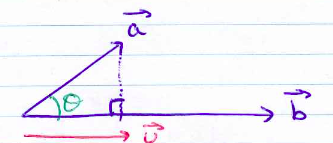
\includegraphics[width=100mm]{assets/lec1_orth.png} 
\end{center}
\[
\left\Vert u \right\Vert = \cos  \left( \theta \right) \left\Vert a \right\Vert 
\]
by trigonometry and so if we want to find what $\vec{u} $ is then we know it's in the direction of $\vec{b} $ so we scale $\vec{b} $ to be a unit vector and then multiply by $\left\Vert u \right\Vert $ that gives
\[
\vec{u} = \left\Vert a \right\Vert \cos  \left( \theta \right) \frac{\vec{b} }{\left\Vert b \right\Vert }
\]

Then the projection of $\vec{a} $ on $\mathit{span} {\vec{b} } $ follows, observe 
\[
    \vec{u} = \left\Vert a \right\Vert \cos  \left( \theta \right) \frac{\vec{b} }{\left\Vert b \right\Vert } \left( \frac{\left\Vert b \right\Vert }{\left\Vert b \right\Vert } \right) = \left\Vert a \right\Vert \left\Vert b \right\Vert \cos  \left( \theta \right) \frac{\vec{b} }{\left\Vert b \right\Vert ^2 }= \frac{a \cdot b}{\left\Vert b \right\Vert ^2 }\vec{b} 
\]

\begin{defn}[Orthogonal Projection]\index{Orthogonal Projection}\label{defn:orthogonal_projection}
    For two vectors $\vec{a} , \vec{b} $ the orthogonal projection is given by
    \[
    \frac{a \cdot b}{\left\Vert b \right\Vert ^2 }\vec{b} 
    \]
\end{defn}

\subsection{Law of Cosines}%
\label{sub:law_of_cosines}
% subsection law_of_cosines

\begin{center}
    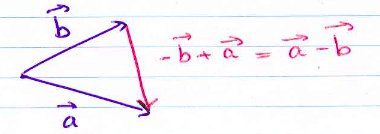
\includegraphics[width=100mm]{assets/lec1_loc.png} 
\end{center}

We have
\[
    \left\Vert a - b \right\Vert ^2 = \left( a - b \right)  \cdot \left( a - b \right) = \left\Vert a \right\Vert ^2  + \left\Vert b \right\Vert ^2  - 2\left( a  \cdot b \right) 
\]
which matches the geometric intuition 

\paragraph{Homework} 

\begin{center}
    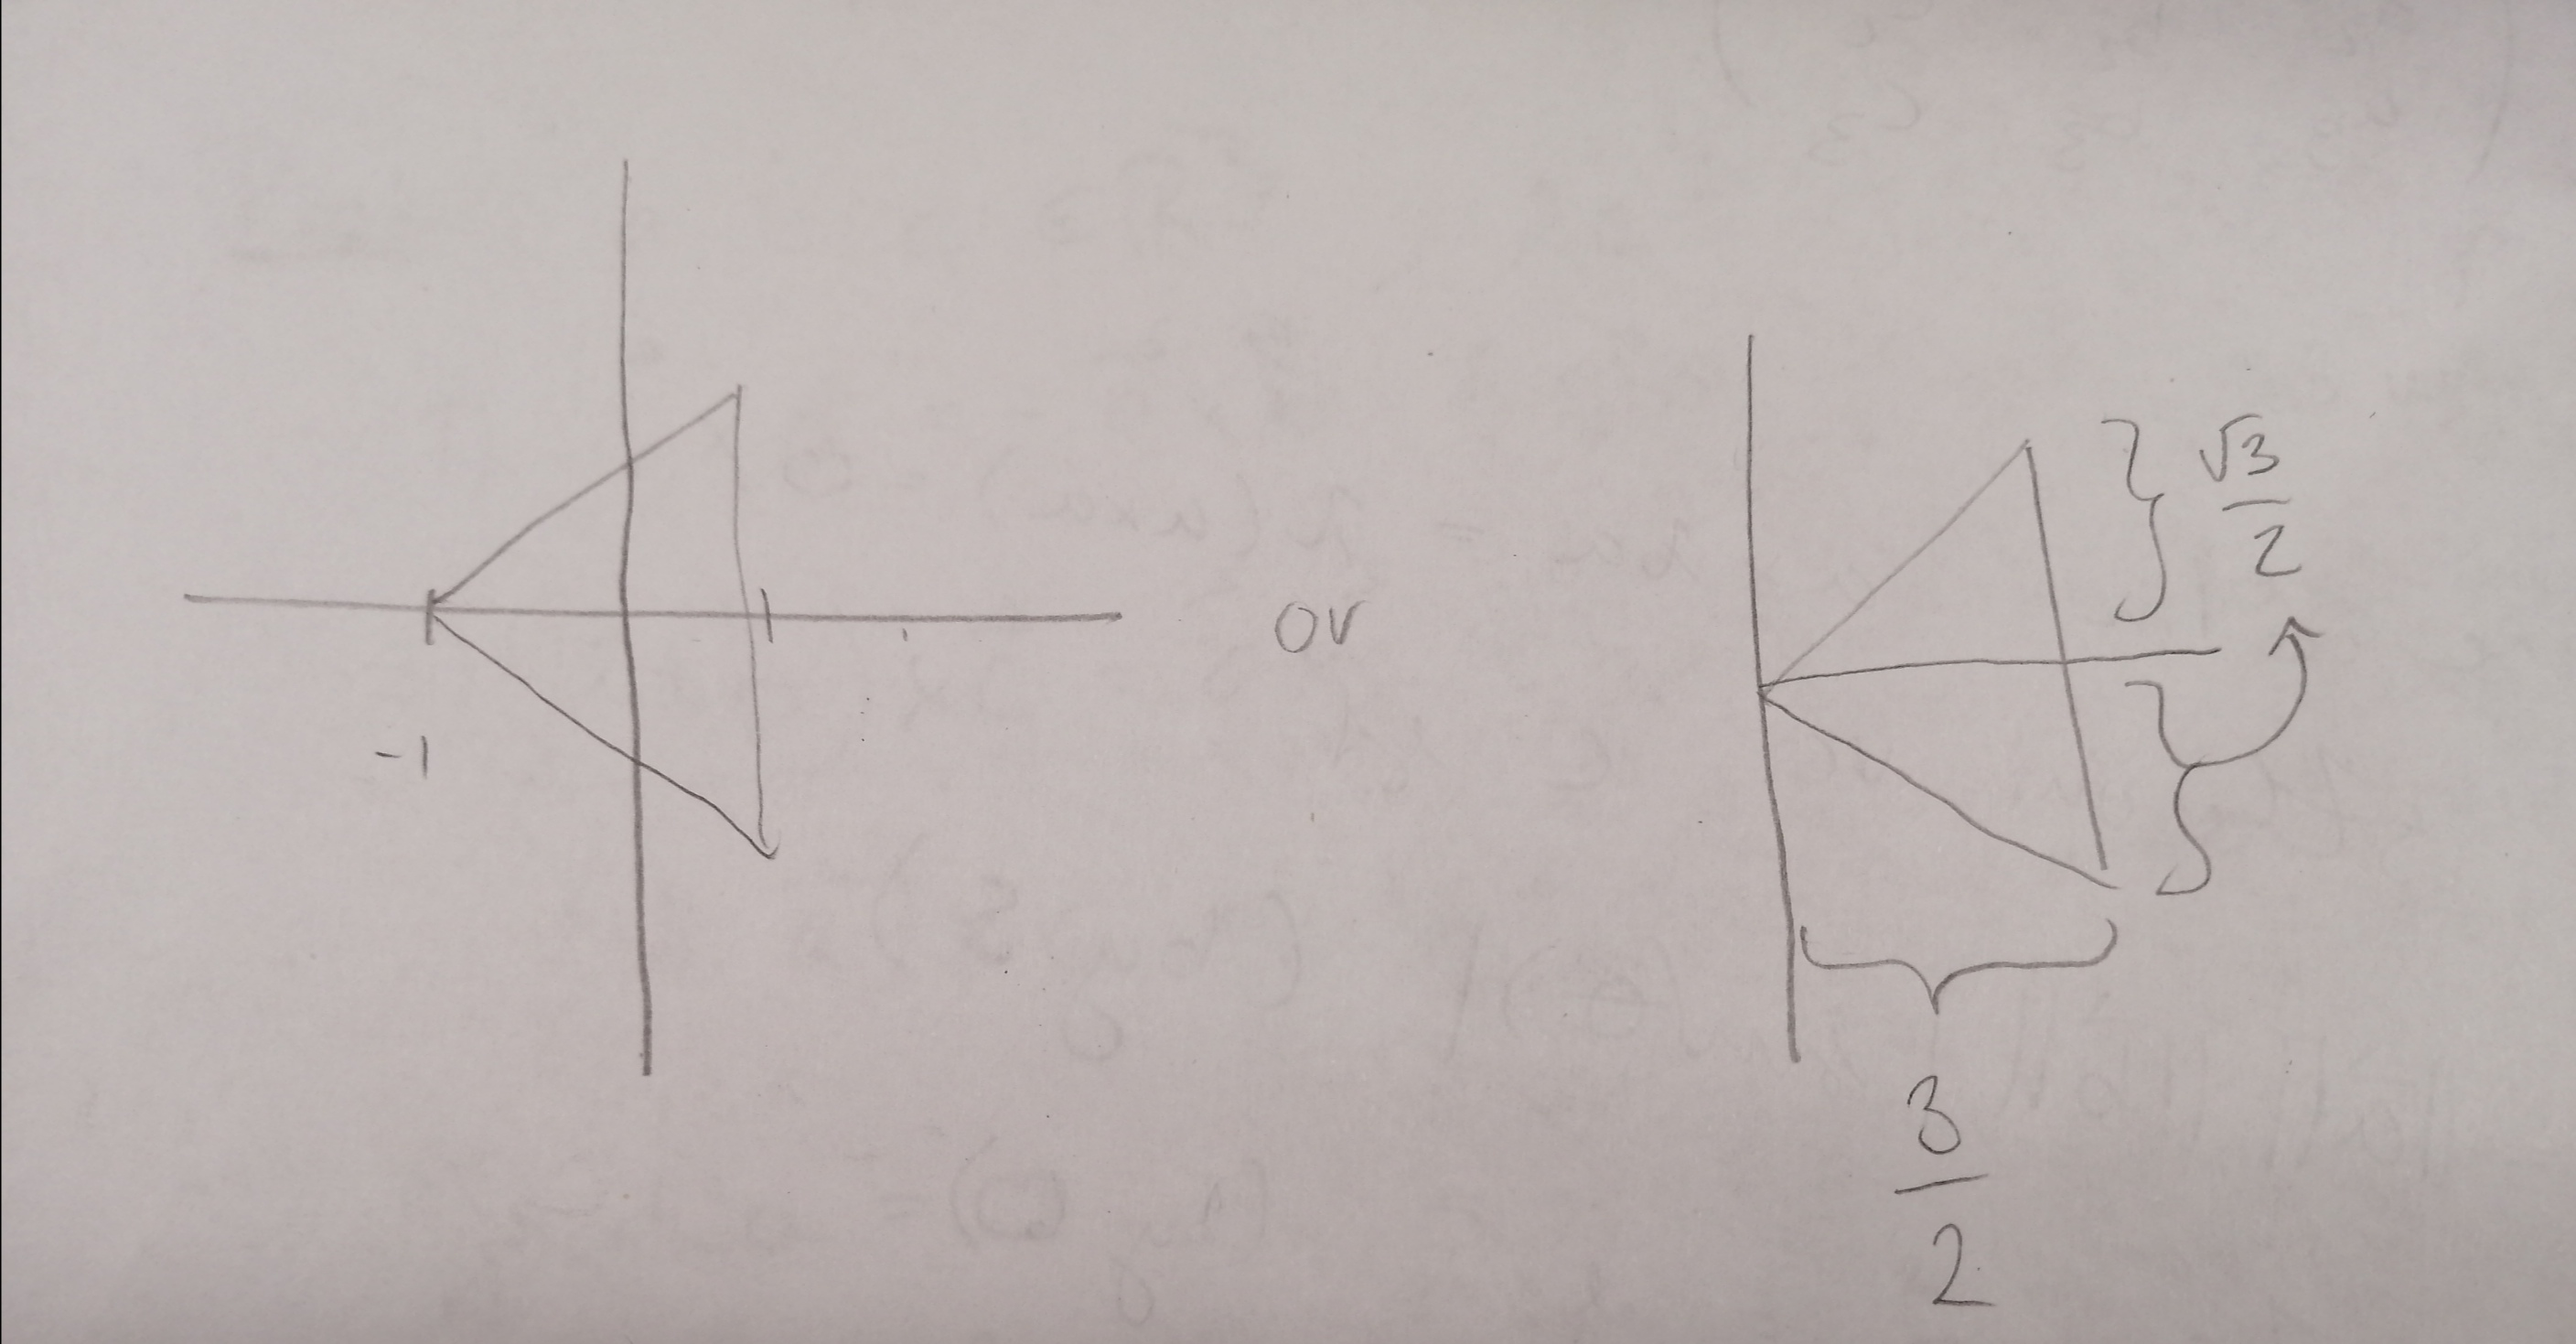
\includegraphics[width=100mm]{assets/lec1_hw.jpg} 
\end{center}

Let $\vec{x} = \vec{AB} \text{ and } \vec{y} = \vec{AC} $, 
\begin{itemize}
    \item Algebraically we have $\vec{x}  \cdot \vec{y} = \left( \frac{3}{2} \right) ^2  + \left( \frac{\sqrt{3} }{2} \right) \left( \frac{ - \sqrt{3} }{2} \right) = \frac{9}{4} - \frac{3}{4}= \frac{6}{4}= \frac{3}{2}$ 
    \item Geometrically, we have $\left\Vert x \right\Vert  \left\Vert y \right\Vert \cos  \left( \theta \right) $,  note $\left\Vert x \right\Vert = \left\Vert y \right\Vert $ and that $\left\Vert x \right\Vert = \sqrt{3} $ so then we have $3\cos  \left( \theta \right) = \frac{3}{2} \Leftrightarrow \cos  \left( \theta \right) = \frac{1}{2}$ so that is if $\theta = \frac{\pi }{6}$ by symetry, we know the other two angles are $\frac{5\pi }{12}$ 
\end{itemize}

% subsection law_of_cosines (end)


\newpage

\begin{defn}[Orthogonality]\index{Orthogonality}\label{defn:orthogonality}
    two vectors $a,b$ are orthogonal if and only if $a \cdot b= 0$ 
\end{defn}
\begin{itemize}
    \item Observe that if we have $\left\Vert u \right\Vert = 1$ then $u$ is a unit vector, and $v$ be any vector, then $\left( u \cdot v \right) u$ is the projection of $v$ onto the line defined by $u$. Since $\left( u \cdot v \right) $ is $\left\Vert u \right\Vert \left\Vert v \right\Vert \cos  \left( \theta \right) $, where $\theta $ is the angle between the two vectors, and that $\left\Vert u \right\Vert = 1$ then $\left( u \cdot v \right) $ is the length of the adjacent side, then multiply a the unit vector which gives the projection.  
    \item If we have $v = v_1 + v_2$ where $v_1$ is parrallel to $u$ and $v_2$ is orthogonal to $u$ then $\left( u \cdot v \right) u$ gives us the projection onto $\vec{u} $ which is just $v_{1} $
        \item $u \cdot v$ is the length of the projection of $v$ onto $u$ which is the same as $v_1 \cdot u$, but recall that $v_1$ and $u$ are paralell, therefore the angle between them is either $0$ or $\pi $,  therefore we have $\left\Vert u \right\Vert \left\Vert v \right\Vert \cos \left( \theta \right) = \pm \left\Vert u \right\Vert \left\Vert v_1 \right\Vert $   
        \item Finally, we form a right triangle with hypotenuse given by $v$ with a base which lies along $u$, then the base is given by $\left( u \cdot v \right) u$ using the same reasoning as in our first observation.
\end{itemize}

\begin{defn}[Norm]\index{Norm}\label{defn:norm}
    Let $a \in \mathbb{R}^{n}  $ 
    \[
    \left\Vert a \right\Vert = \sqrt{a \cdot a} = \sqrt{a_{1}^2   +  a_{2}^2   +  \dotsb   +  a_{n - 1}^2   +  a_{n}^2  } 
    \]
    geometrically this is the length of $a$, also $\left\Vert a - b \right\Vert $ is the distance between $a \text{ and } $ 
\end{defn}


% subsection operations_on_n_tuples (end)

\subsection{Important properties of the norm}%
\label{sub:important_properties_of_the_norm}
% subsection important_properties_of_the_norm

Prove the following.
\begin{enumerate}
    \item $\left\Vert a \right\Vert \ge 0$ 
    \item $\left\Vert a \right\Vert = 0 \implies a = \vec{0} $ 
    \item $\left\Vert \lambda a \right\Vert = \left| \lambda  \right| \left\Vert a \right\Vert  $ 
    \item $\left\Vert a + b \right\Vert \le \left\Vert a \right\Vert  + \left\Vert b \right\Vert $, (hint use 5)
    \item $\left| a \cdot b \right| \le \left\Vert a \right\Vert \left\Vert b \right\Vert $ (Cauchy-Schwarts inequality)
    \item $a \cdot e_{j} = a_{j} $ 
    \item $e_{j}  \cdot e_{j} = 1$ 
    \item for $i\neq j$,  $e_{j}  \cdot e_{i} = 0$ 
    \item $a \cdot b = \frac{1}{4}\left( \left\Vert a + b \right\Vert ^2  - \left\Vert a - b \right\Vert ^2  \right) $ (Polarization identity )
\end{enumerate}

\underline{Proofs} 

\begin{enumerate}
    \item $\left\Vert a \right\Vert \ge 0$
        \begin{proof}
        $ $\newline
            $\forall x \in \mathbb{R} , x^2 \ge 0 \implies \sum_{i=0}^{n} a_{i} ^2 \ge 0 \implies \sqrt{\sum_{i=0}^{n} a_{i} ^2  } \ge 0 \Leftrightarrow \left\Vert a \right\Vert \ge 0$
        \end{proof}
    \item $\left\Vert a \right\Vert = 0 \implies \vec{a} = \vec{0} $
        \begin{proof}
        $ $\newline
            Assume $\left\Vert a \right\Vert = 0$, for contradiction we assume $\exists i \in \left\{ 1, \ldots , n \right\} \text{ such that } a_{i} \neq 0 $  then $\sqrt{\sum_{i=0}^{n} a_{i} ^2}  \neq 0 \Leftrightarrow \left\Vert a \right\Vert \neq 0$ thus we have a contradiction therefore $a = \vec{0} $.  
        \end{proof}
    \item $\left\Vert \lambda a \right\Vert = \left| \lambda  \right| \left\Vert a \right\Vert $ 
    \begin{proof}
    $ $\newline
    We commence ,
    \begin{align*}
        \left\Vert \lambda a \right\Vert &= \sqrt{\sum_{i=0}^{n} \left( \lambda a_{i}  \right) ^2  } \\
        &= \sqrt{\lambda ^2 \sum_{i=0}^{n} a_{i} ^2  }   \\ 
        &= \lambda \sqrt{\sum_{i=0}^{n} a_{i} ^2  }   \\ &= \lambda \left\Vert a \right\Vert   \\ 
    \end{align*}
    \end{proof}
    \item $\left\Vert a + b \right\Vert \le \left\Vert a \right\Vert  + \left\Vert b \right\Vert $ 
    \item $\left| a \cdot b \right| \le \left\Vert a \right\Vert \left\Vert b \right\Vert $ 
    \begin{proof}
    $ $\newline
    We will commense with left hand side 
        \begin{align*}
            \left\Vert a + b \right\Vert &= \left\Vert \left( a_1 + b_1, \ldots ,  + a_{n}  + b_{n}  \right)  \right\Vert   \\ 
            &= \sqrt{\left( a_{1}  + b_1 \right)^2  + \ldots  + \left( a_{n}  + b_{n}  \right) ^2  }   \\ 
            &= \sqrt{\left( a_1^2  + 2a_1b_1 + b^2  \right)  + \ldots  + \left( a_{n} ^2  + 2a_{n} b_{n}  + b_{n} ^2  \right) }   \\ 
            &= \sqrt{\sum_{i=1}^{n} a_{i} ^2  + \sum_{i=1}^{n} b_{i} ^2  + 2\left( a \cdot b \right)   }   \\ 
            &\le    \sqrt{\sum_{i=1}^{n} a_{i} ^2  + \sum_{i=1}^{n} b_{i} ^2  + 2\left| a \cdot b \right|     }   \\ 
            \intertext{From 5, it follows that } 
            &\le     \sqrt{\sum_{i=1}^{n} a_{i} ^2  + \sum_{i=1}^{n} b_{i} ^2  + 2\left( \left\Vert a \right\Vert \left\Vert b \right\Vert  \right)     }   \\ 
            &= \sqrt{\left\Vert a \right\Vert ^2  + \left\Vert b \right\Vert ^2  + 2\left\Vert a \right\Vert \left\Vert b \right\Vert }   \\ 
            &= \sqrt{\left( \left\Vert a \right\Vert  +  \left\Vert b \right\Vert  \right)^2  }  \\ 
            &= \left\Vert a \right\Vert  + \left\Vert b \right\Vert    \\ 
        \end{align*}
        Therefore 
        \[
        \left\Vert a + b \right\Vert \le \left\Vert a \right\Vert  + \left\Vert b \right\Vert 
        \]
        as required
    \end{proof}
    \begin{proof}
    $ $\newline
        Let $f\left(t\right) = \left\Vert a + tb \right\Vert ^2 $, for $t \in \mathbb{R}, a, b \in  \mathbb{R} ^{n}  $  
\begin{align*}
    \left\Vert a + tb \right\Vert ^2 &= \left( a + tb \right) ^2 
    \\ 
    &= \left( a \cdot a \right)  + 2\left( a \cdot tb \right)  + \left\Vert b \right\Vert ^2 t^2 
\end{align*}
    observe we have a quadratic polynomial whose leading coefficient is non-negative, and that $f\left(t\right) \ge 0$ since the norm of any vector is non-negative. Therefore it can have at most one solution, that is only if the inner part of the descriminant is less than or equal to 0
    \[
    \sqrt{b^2  - 4ac} \le 0
    \]
    though in our case we have, using the fact that $\sqrt{x^2 } = \left| x \right| $ 
    \begin{gather*}
        \sqrt{4\left( a \cdot b \right) ^2 }  - 4\left\Vert a \right\Vert ^2 \left\Vert b \right\Vert ^2 \le 0\\
        4\left( a \cdot b \right) ^2  - 4\left\Vert a \right\Vert ^2 \left\Vert b \right\Vert ^2 \le 0\\
        \left( a \cdot b \right) ^2 \le \left\Vert a \right\Vert ^2 \left\Vert b \right\Vert ^2 \\
        \left| a \cdot b \right| \le \left\Vert a \right\Vert \left\Vert b \right\Vert 
    \end{gather*}
    \end{proof}
    \item We will prove $a \cdot e_{j} = a_{j} $ 
        \begin{proof}
        $ $\newline
        we have $e_{j} = \left( 0, \ldots , 1, \ldots , 0 \right) $ where $1$ is at the $j$-th entry then in the dot product we have 
        \begin{align*}
            a \cdot e_{j} = \sum_{i=1}^{n} a_{i} e_{j,i} = 0  + \ldots  + a_{j} \left( 1 \right)  + \ldots  + 0=  a_{j} 
        \end{align*}
        \end{proof}
    \item We will prove $e_{j}  \cdot e_{j} = 1$ 
        \[
            e_{j}  \cdot e_{j} = 0  \cdot 0  +  \ldots   + 1 \cdot 1  + 0 \cdot 0 \ldots  + 0 \cdot 0 = 1
        \]
    \item We will prove for $i \neq j, e_{j}  \cdot e_{i} = 0$ 
        We know that zero multiplied by anything is also 0, therefore the only chance that this sum is non-zero, is if $e_{j} \text{ and } e_{i} $ would have a non-zero value at the same entry, though by construction, it does not, therefore $e_{j}  \cdot e_{i} = 0$.
\end{enumerate}

% subsection important_properties_of_the_norm (end)


\begin{defn}[Subspace]\index{Subspace}\label{defn:subspace}
    a subspace of euclidiean space $\mathbb{R} ^{n} $ is a set $V$ such that, if $a, b \in V$ then $c_1a + c_2b \in V$ for all $c_1, c_2\in  \mathbb{R} $. Observe, that $\vec{0} \in V$ always. 
\end{defn}

suppose A is $m\times n$ matrix 
\begin{itemize}
    \item If each of the $n$ columns of $A$ are linearly independent, then $\left\{ Ax: x \in  \mathbb{R} ^{n}  \right\} $ spans all of $n$ dimensional space, we call the subspace consisting of all the linear combinations of $A$ the column space or image of $A$.
    \item take $m = 3 \text{ and } n= 2$, then we get a plane spanned by the two column vectors of $A$ assuming they are linearly independent. 
    \item If each of the $m$ rows of $A$ are linearly independent, then $\left\{ x \in \mathbb{R} ^{n} : Ax= 0 \right\} $ is $\left( m - n \right) $ dimensional, since by the Rank Nullity Theorem, we know that the dimension of the null space added to the rank, gives $n$. Observe, that this is the sub space of vectors that are orthogonal to every row of $A$ by the way that matrix vector multiplication is defined.  Say we have $m= 2 \text{ and } n = 3$ then the null space must be orthogonal to both of the row vectors who define a plane, and the null space is orthognal to every point on this plane.
\end{itemize}

\newpage

\begin{defn}[Cross Product]\index{Cross Product}\label{defn:cross_product}
    Only in $\mathbb{R} ^{3} $ we have a different way of multiplying two vectors. For $a, b$,  the cross product (a vector) denoted as $a\times b$ id defined, algebraically by 
    \[
        a\times b= \left( a_2b_3 - a_3b_2, a_3b_1 - a_1b_3, a_1b_2 - a_2b_1 \right) 
    \]
    Geometrically, $a\times b = \vec{0} $ if $a, b$ are linearly dependent , otherwise it is the unique vector that is orthogonal to both $a \text{ and } b$ with length given by
    \[
        \left\Vert a\times b \right\Vert ^2 = \left\Vert a \right\Vert ^2 \left\Vert b \right\Vert ^2  - \left( a \cdot b \right) ^2 
    \]
    so that the parallelpiped formed by $a, b \text{ and } a\times b$ is positively oriented.
\end{defn}

We can verify that the definitions are the same algebraically, that $a  \cdot \left( a\times b \right) = 0$ and $b \cdot \left( a\times b \right) = 0$ 
\begin{align*}
    a \cdot \left( a\times b \right) &= a_1a_2b_3 - a_1a_3b_2 + a_2a_3b_1 - a_2 a_1 b_3 + a_3a_1 b_2 - a_3a_2b_1 = 0 \\ 
\end{align*}

$\left\Vert a\times b \right\Vert ^2 = \left\Vert a \right\Vert ^2 \left\Vert b \right\Vert ^2  - \left( a \cdot b \right) ^2 $, computations follow 
The determinant of $[a, b, a\times b]$ turns out to be the sum of squares...

To recall the definition for the cross product we can use the following diagram
\begin{center}
    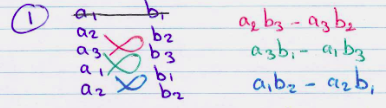
\includegraphics[width=100mm]{assets/lec1_cp.png} 
\end{center}

\subsection{Properties of the Cross Product}%
\label{sub:properties_of_the_cross_product}
% subsection properties_of_the_cross_product

\begin{itemize}
    \item $a\times b =  - \left( b\times a \right) $
    \item $\left( cx + dy \right)\times z = \left( cx \times z \right)  + \left( dy\times z \right)  $ where $c, d \in \mathbb{R} $ 
    \item $\left\Vert a\times b \right\Vert = \left\Vert a \right\Vert \left\Vert b \right\Vert \sin  \left( \theta \right) $ that is the length of $a\times b$ is equal to the area of the parallelogram generated by $a \text{ and } b$  
        \item The cross product is not associative, observe 
            \[
                \left( i\times i \right) \times j = 0 
            \]
            But 
            \[
                i \times \left( i\times j \right) =  - j
            \]
            
\end{itemize}

\paragraph{From Lecture} 
\begin{enumerate}
    \item $b\times a =  - \left( a\times b \right) $ 
    \item $\left( \lambda a + b \right) \times c = \lambda \left( a\times b \right)  + b\times c$ 
    \item $a\times a = 0$ 
    \item $\left\Vert a\times b \right\Vert^2  + \left( a \cdot b \right) ^2 = \left\Vert a \right\Vert ^2 \left\Vert b \right\Vert ^2 $ 
    \item $\left\Vert a\times b \right\Vert = \left\Vert a \right\Vert \left\Vert b \right\Vert \left| \sin  \left( \theta \right)  \right| $ 
    \item $a \cdot \left( a\times b \right) = 0 \text{ and } b \cdot \left( a\times b \right) = 0$ 
    \item $i\times j= k, j\times k= i, k\times i= j$ 
    \item $a\times \left( b\times c \right) = \left( a \cdot b \right) b - \left( a \cdot b \right) c$ also $\left( a\times b \right) \times c = \left( a \cdot c \right) b  -  \left( b - c \right) a$ 
    \item $a\times \left( b\times c \right)  + b\times \left( c\times a \right)  + c \times \left( a\times b \right) = 0$ 
    \item $\left( a\times b \right)  \cdot c = \mathit{det} \left(
            \begin{bmatrix}
            	a_{1}  &b_{1}   & c_{1}  \\
            	a_{2}  &b_{2}   & c_{2}  \\
            	a_{3}  &b_{3}   & c_{3}  
            \end{bmatrix}
        \right) $ 
\end{enumerate}

\todo{Add rest of lecture here} 

% subsection properties_of_the_cross_product (end)

% section geometry_in_higher_dimensions (end)

% chapter lecture_2 (end)

\chapter{Lecture 3}%
\label{chp:lecture_3}
% chapter lecture_3


% chapter lecture_3 (end)

\section{Visualizing Mult-Var}%
\label{sec:visualizing_mult_var}
% section visualizing_mult_var

consider $f : \mathbb{R} ^2  \to \mathbb{R}  $ 
\begin{itemize}
    \item We have the graph, that is 
        \[
            \left\{ \left( x,y, z \right) \in  \mathbb{R} ^{3} : z= f\left(x, y\right)  \right\}    
        \]
        Observe this yields a two-dimensional surface, with a given height $z$ over a point $\left( x,y \right) $ 
\end{itemize}

\begin{defn}[Level Curve]\index{Level Curve}\label{defn:level_curve}
    For $c \in  \mathbb{R} $,  the level curve (level set or contour plot ) of $f : \mathbb{R} ^2  \to R $ is 
    \[
        \left\{ \left( x, y \right) \in \mathbb{R} : f\left(x,y\right) = c \right\} 
    \]
\end{defn}

Observe, we have the 3d graph of $f\left(x, y\right) = \frac{1}{9}x^2  + \frac{1}{4}y^2 $  

\begin{center}
    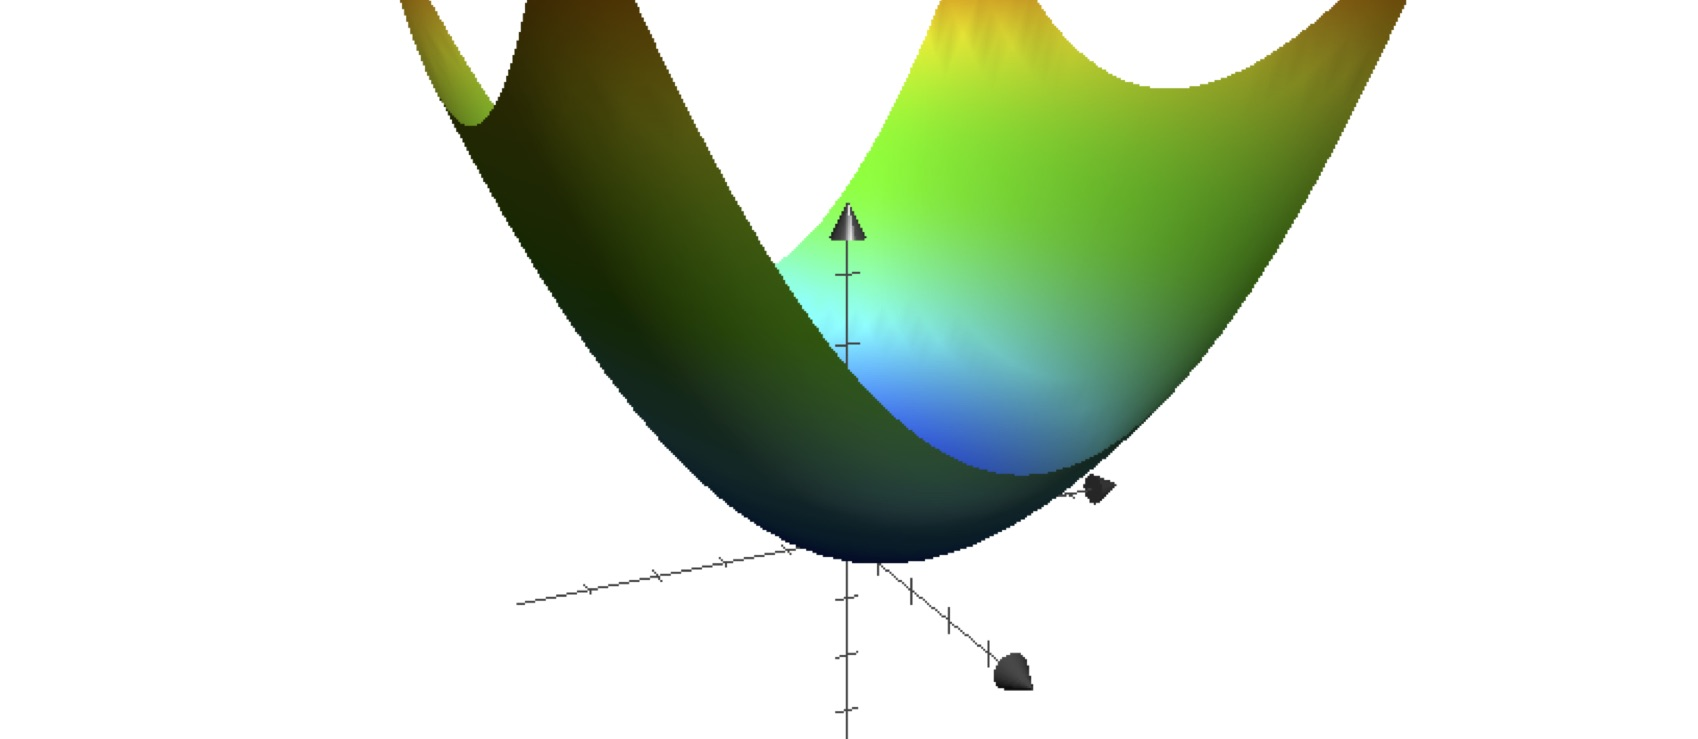
\includegraphics[width=0.7\columnwidth]{assets/3d-graph.jpg}
\end{center}

Then the level curve of the same function 

\begin{center}
    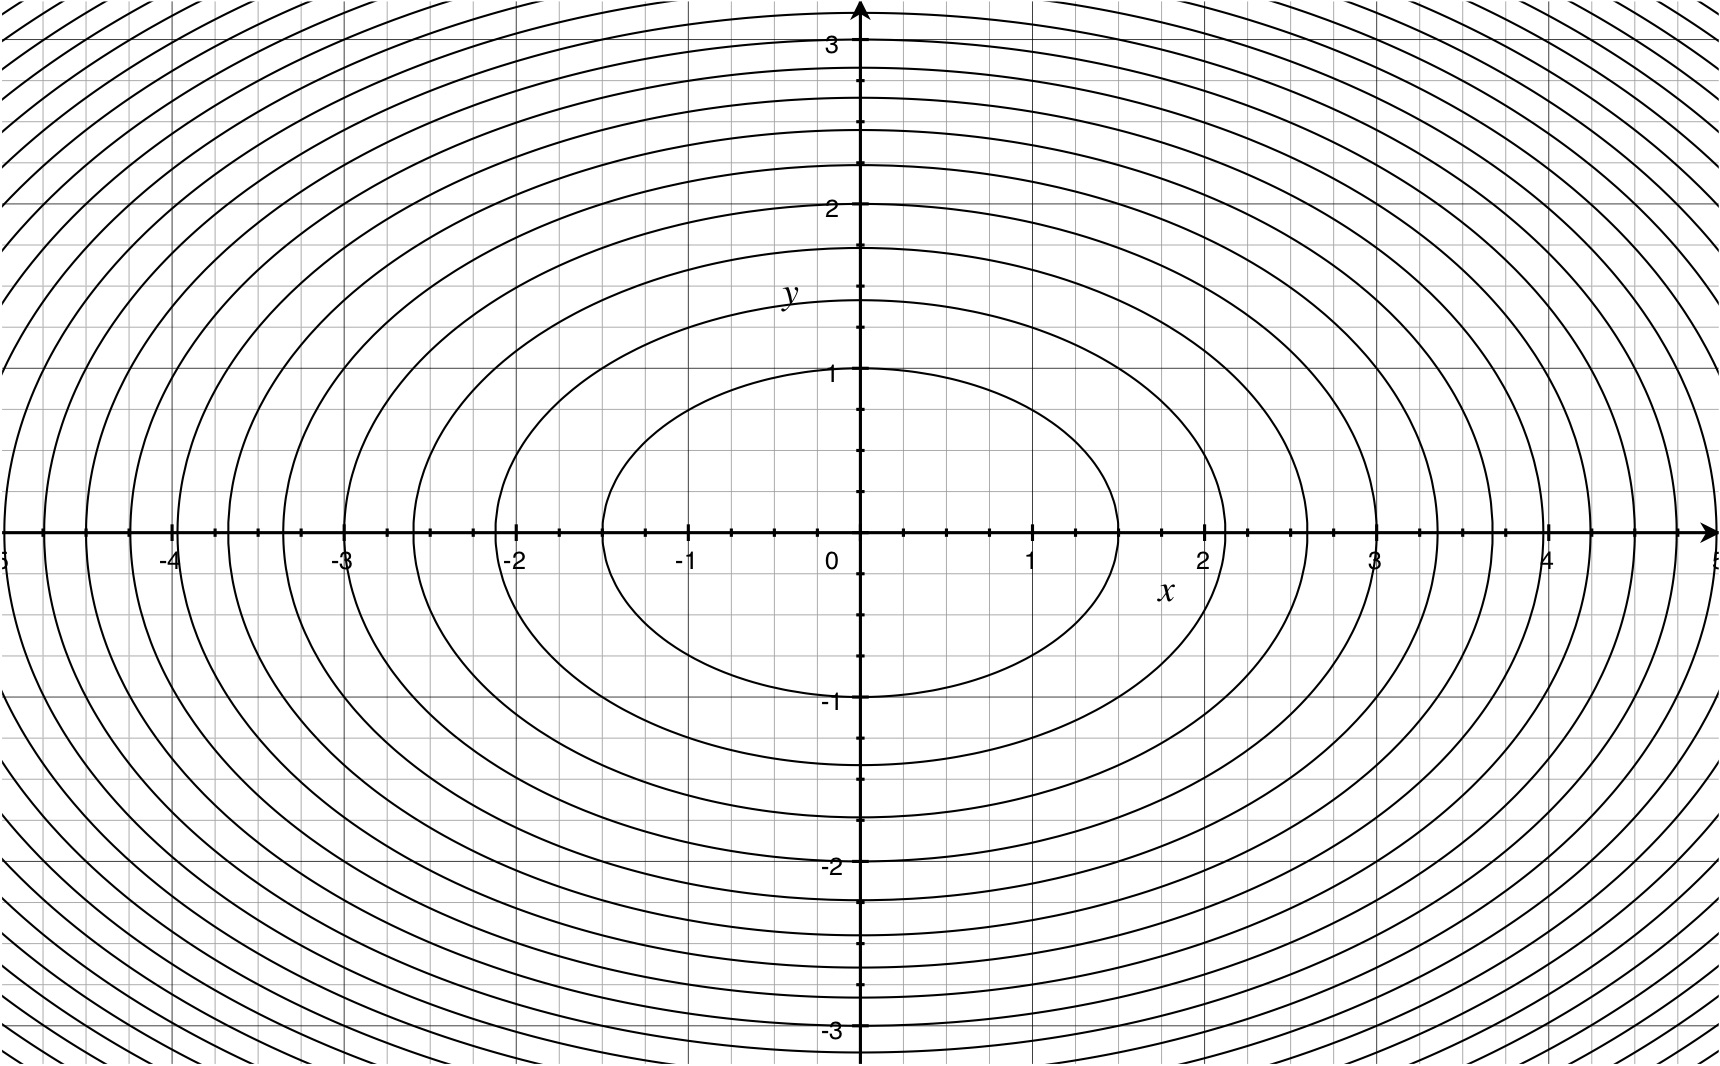
\includegraphics[width=0.7\columnwidth]{assets/level-c.jpg} 
\end{center}

Note that the values of $c$ are chosen to be evenly spaced, thefeore we can observe when the curves are closer together we can see that the function changes faster.

\subsection{Level Curve Questions - Online}%
\label{sub:level_curve_questions_online}
% subsection level_curve_questions
We'll match the graph to the level curve.
\begin{itemize}
    \item for the first graph we note that it has flat sides, therefore if we were to slice through it, we will obtain squares, therefore this matches to the 2nd level curve
    \item The second has flat sides, with curved edges, therefore, though it's rotated $\frac{\pi}{2} $ from the previous graph, therefore this matches to the second last graph.
    \item The third graph is similar to the first though it has been pinched on the corners, therefore the contour plot, is the one that is similar ot the second, with the pinch, so we conclude that it is the last contour plot
    \item We see that the fourth graph is similar to the first, though it's sides are softer, so we conclude it matches to the first graph
    \item The last grpah looks like a cone, since it has no corners, therefore if we slice through it we should obtain circles, so the correct contour plot is the third.
\end{itemize}

\newpage

\subsection{Mountains and Valleys - Lecture}%
\label{sub:mountains_and_valleys_lecture}
% subsection mountains_and_valleys_lecture

We note we are taking slices of of the mountains one at a time, and so just like slicing through a cone, if we observe concentric circles that decrease in radius it is most likely a mountain, if we can see that the elevation is increasing then it is for sure.

\begin{center}
    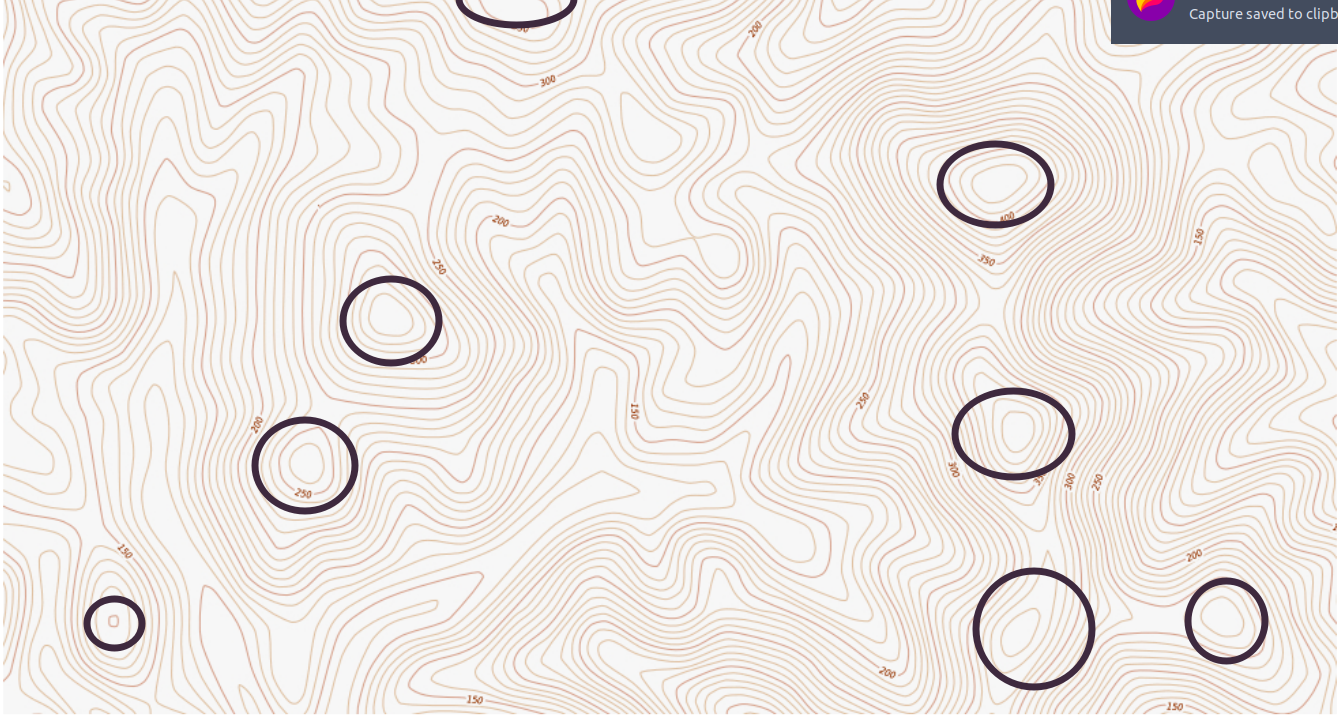
\includegraphics[width=100mm]{assets/lec2_mount.png} 
\end{center}

% subsection mountains_and_valleys_lecture (end)

\subsection{Level Curve Harder}%
\label{sub:level_curve_harder}
% subsection level_curve_harder

Find some level curves of $f\left(x,y\right) = y^2  - x^2 $ 
\[
    f\left(x,y\right) = y^2  - x^2 = \left( y + x \right) \left( y  - x \right) 
\]

We then make a change of variable so 
\begin{align*}
    u = y  - x && v= y + x
\end{align*}
\todo{Understand and complete this} 


% subsection level_curve_harder (end)

% subsection level_curve_questions (end)

\subsection{3-Variable Functions}%
\label{sub:3_variable_functions}
% subsection 3_variable_functions

consider $f : \mathbb{R} ^{3}  \to \mathbb{R} $ a graph can still make sense: 
\[
    \left\{ \left( x,y,z,w \right) \in \mathbb{R} ^{4} : w= f\left(x,y,z\right)  \right\} 
\]
this s a 3 dimensional shape sitting inside 4-dimensional space and is very hard to visualize, therefore we can use a level set to attempt to describe it, that is 
\[
    \left\{ \left( x,y,z \right) \in  \mathbb{R}^{3} : f\left( x,y,z \right) = c \right\} 
\]
for different choices of $c$. We call these a level surface since they are 3-dimensional and let us visuzlize them easier, for the function $f\left(x,y,z\right) = \frac{1}{9}x^2  - \frac{1}{4}y^2  + \frac{1}{9}z^2 $,  the level surface for $c= -2$ is given below

\begin{center}
    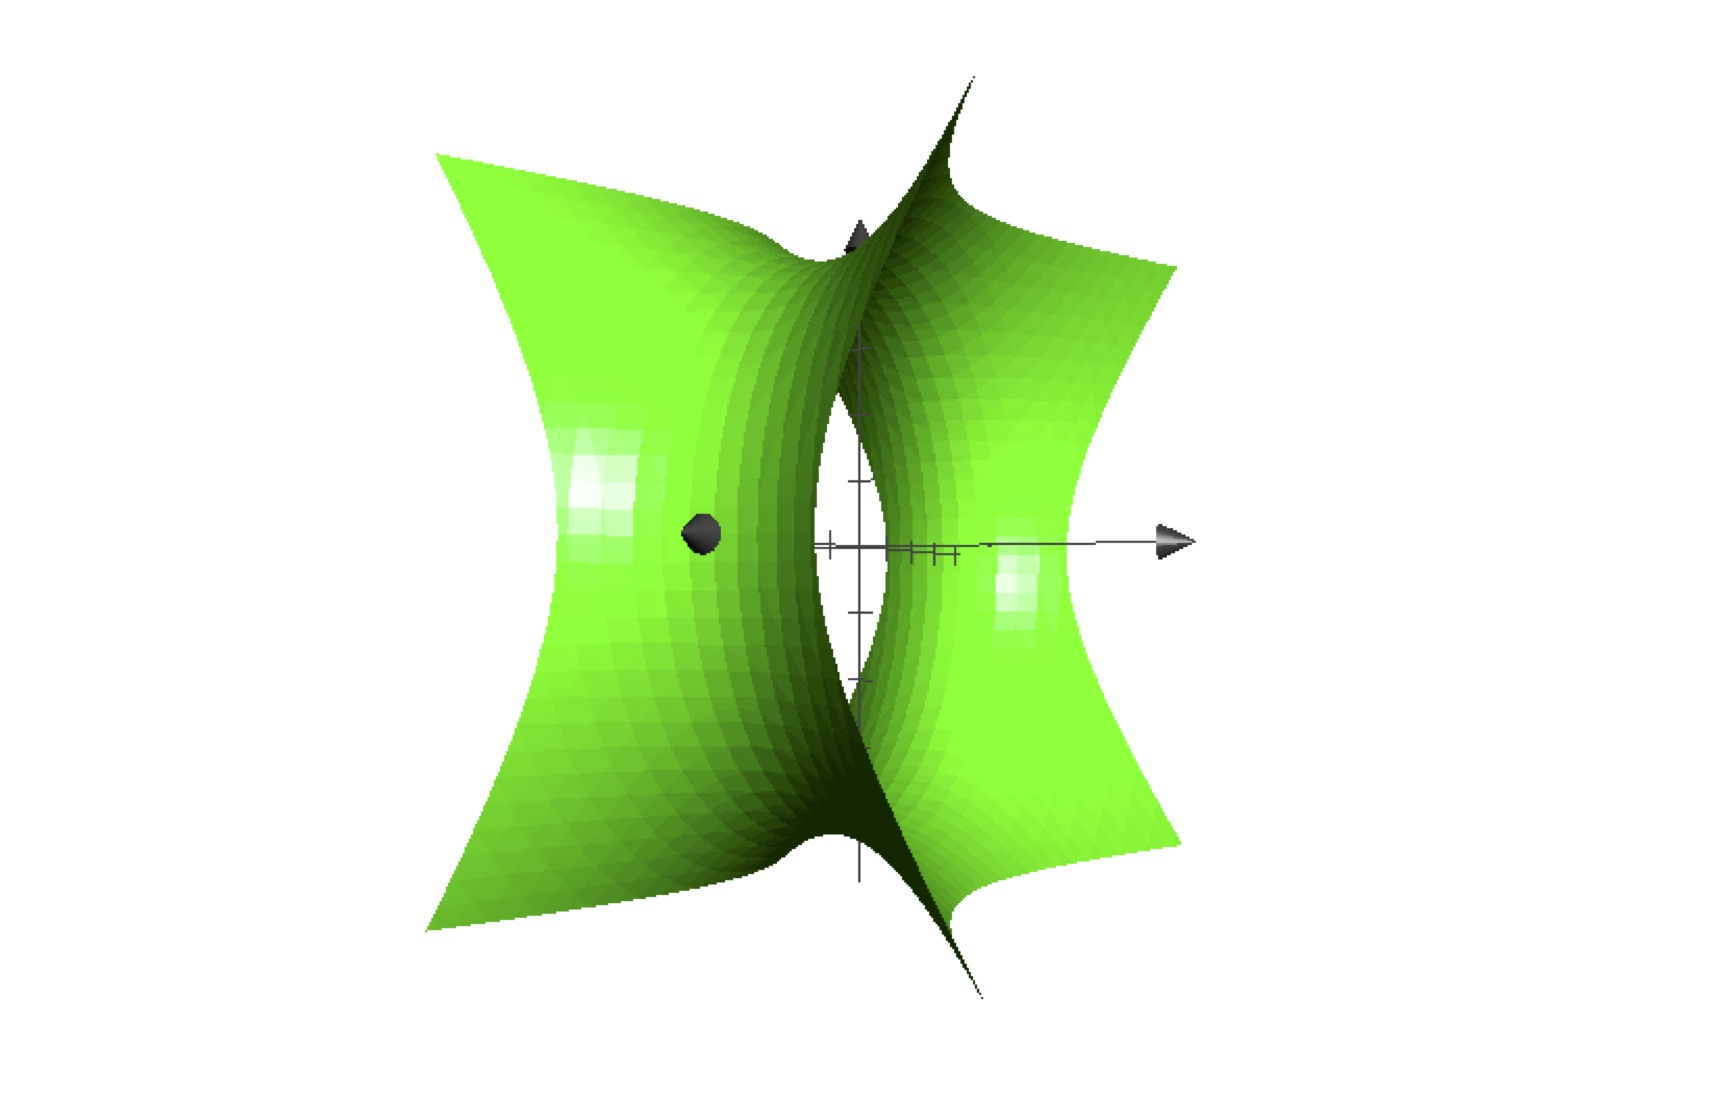
\includegraphics[width=\textwidth]{assets/-2-surf.jpg} 
\end{center}

Sometimes the level surfaces can be written in the form $z=f(x,y)-c$, and you can picture them as shifted graphs of a function of two variables. This situation is the simplest possible, so it may help you visualize what happens in higher dimensions, but it is rare.

\todo{What does this even mean?} 

% subsection 3_variable_functions (end)

\subsection{4 or more}%
\label{sub:4_or_more}
% subsection 4_or_more

We can still define a graph for the function $f : \mathbb{R} ^{n}  \to \mathbb{R}  $ 
\[
    \left\{ \left( x_{1} , x_{2} , \dotsc  , x_{n } , x_{n + 1}  \right) \in \mathbb{R} ^{n + 1} : x_{n + 1} = f\left(x_{1} , x_{2} , \dotsc  , x_{n - 1} , x_{n} \right)   \right\} 
\]

And also the level set
\[
    \left\{ \left( x_{1} ,  x_{2} ,  dotsc ,  x_{n - 1} ,  x_{n}  \right) \in \mathbb{R} ^{n} : f\left(x_{1} , x_{2} , \dotsc  , x_{n - 1} , x_{n} \right) = c \right\} 
\]
Though it's impossible to imagine these for $n\ge 4$. 


% subsection 4_or_more (end)

% section visualizing_mult_var (end)

\section{Topology}%
\label{sec:topology}
% section topology

\begin{defn}[Open Ball]\index{Open Ball}\label{defn:open_ball}
    Let $a \in R^{n} $, $r \in \mathbb{R} > 0$,  the open ball centered at $a$ with radius $r$ is
    \[
    B\left(a, r\right) \coloneqq \left\{ x\in \mathbb{R} ^{n} : \left\Vert a - x \right\Vert \le r \right\} 
    \]
\end{defn}

\paragraph{Example} 
\begin{itemize}
    \item $B\left(\left( 1,2 \right) 1\right) \subseteq \mathbb{R} ^2 $ 
    \begin{center}
        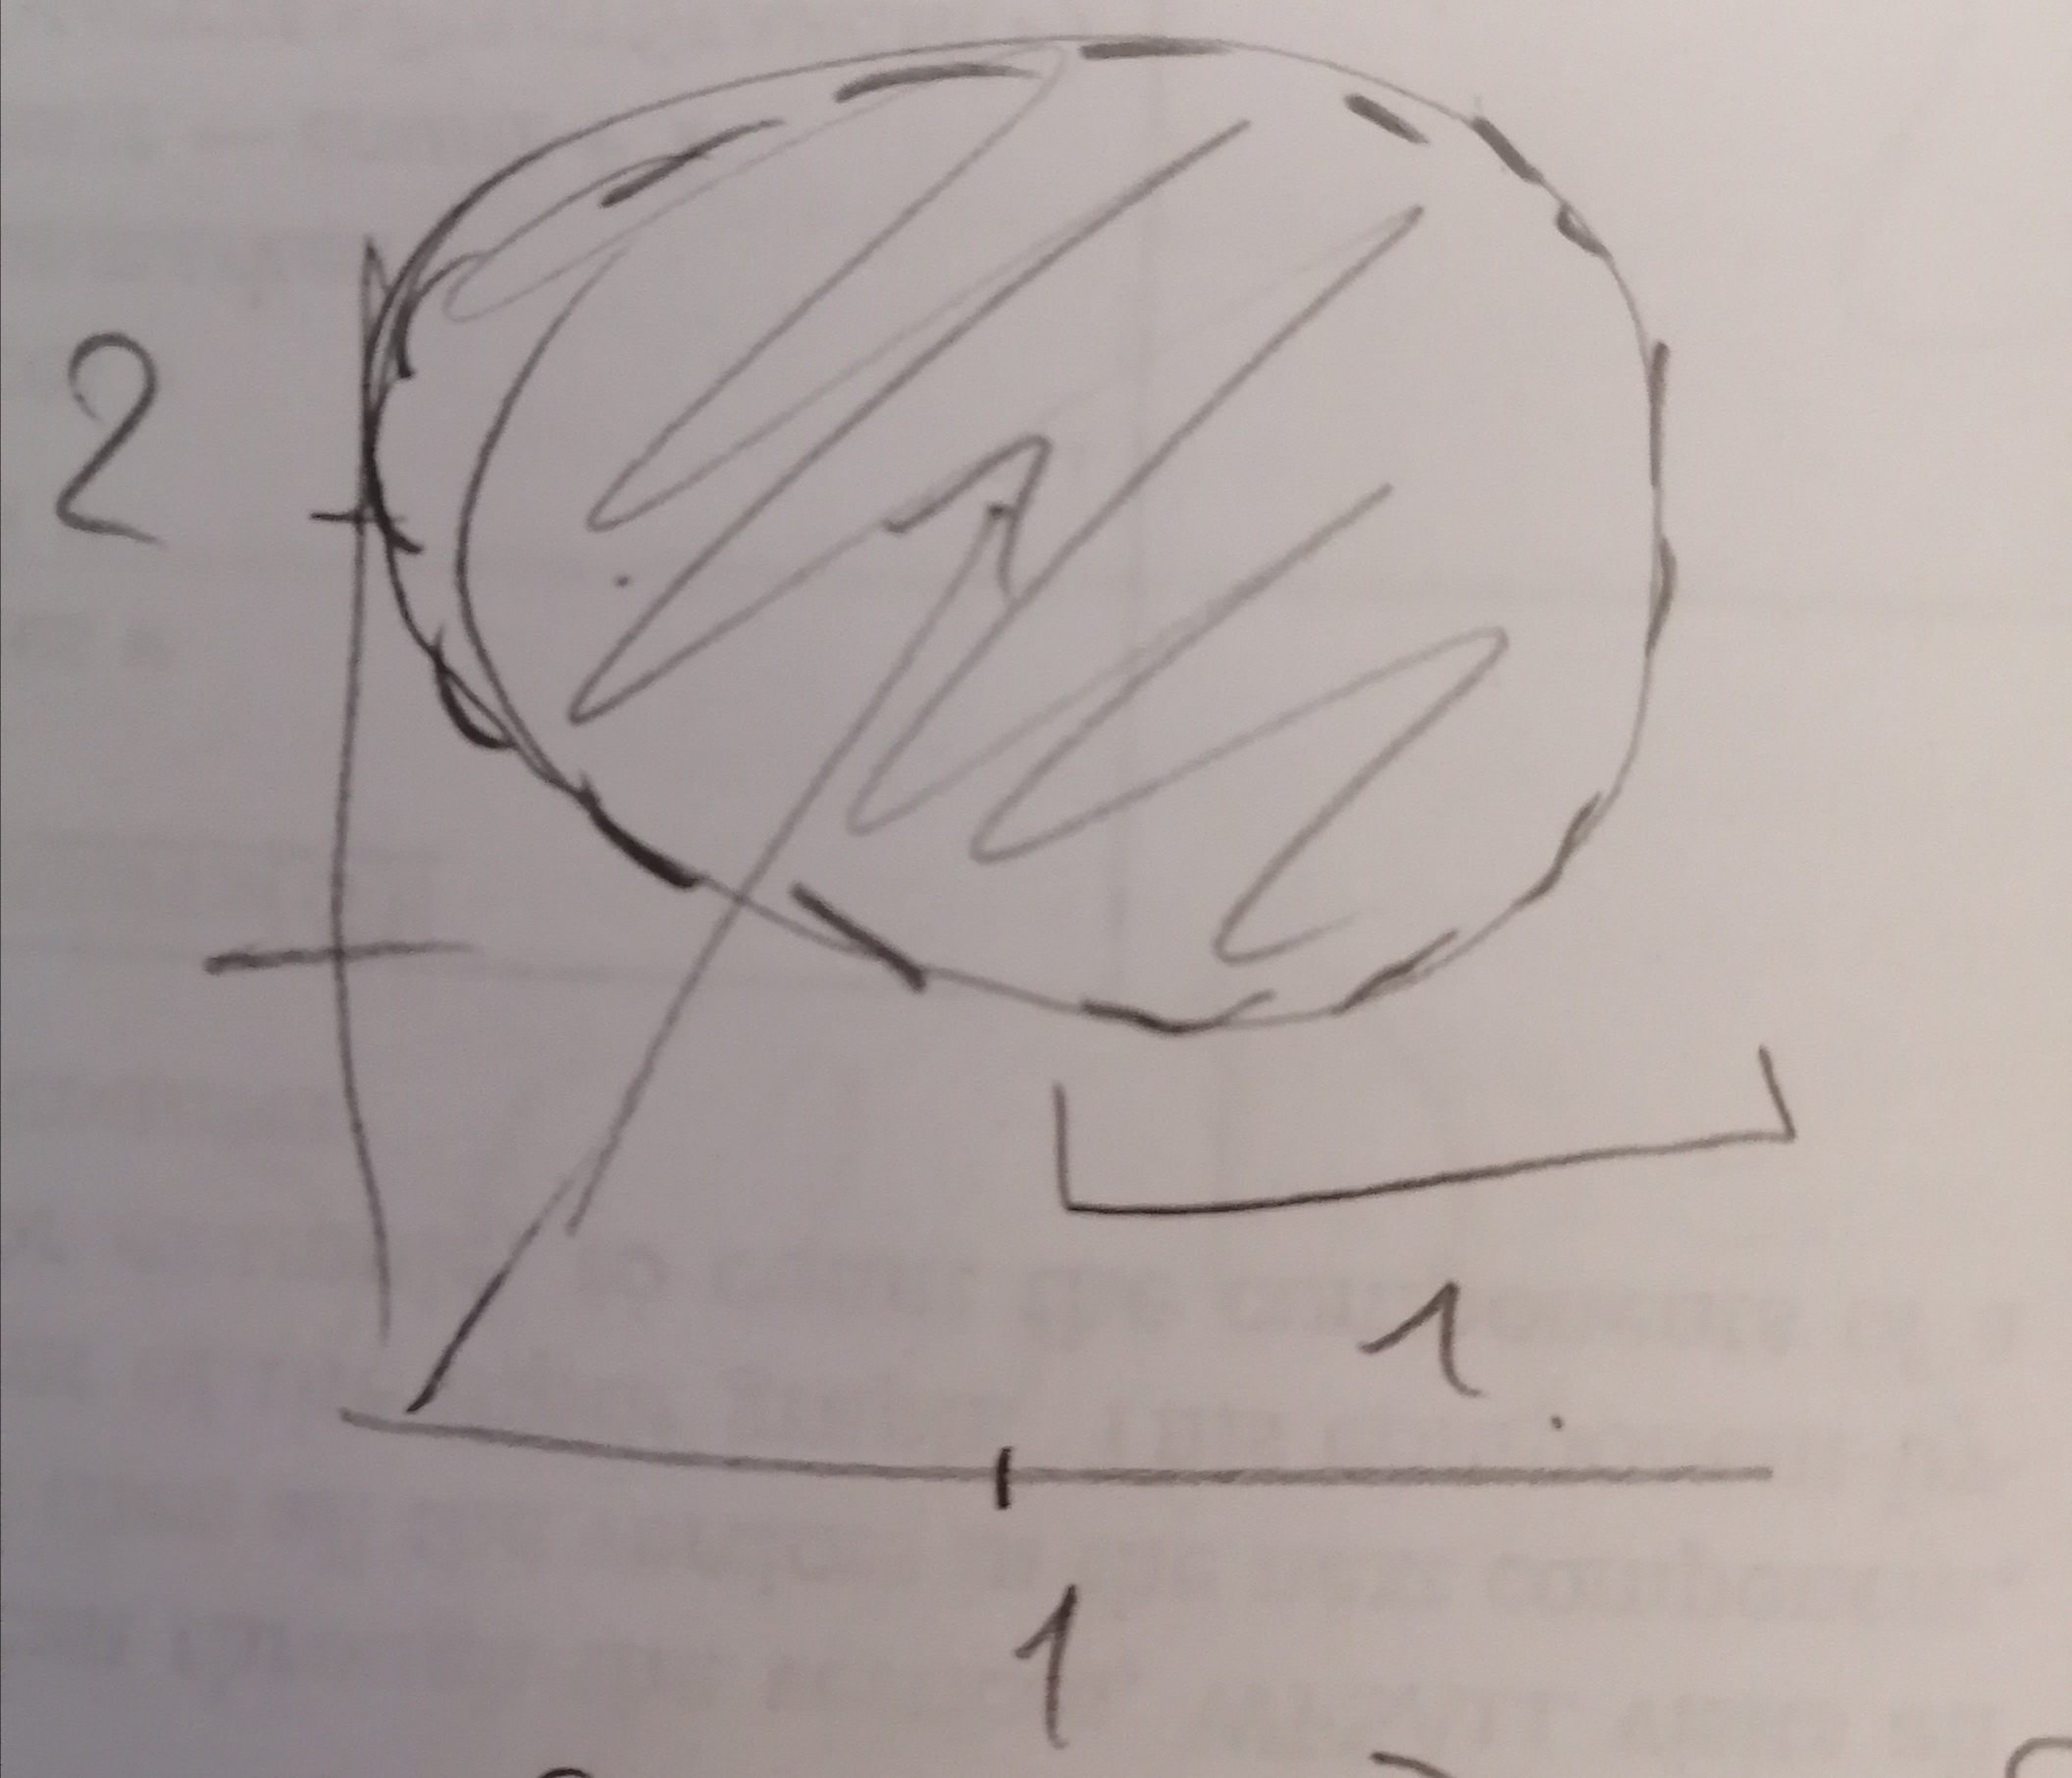
\includegraphics[height=50mm]{assets/lec3_ball-ex.jpg} 
    \end{center}
    \item $B\left(2, 1\right) = \left( 1,3 \right)\subseteq \mathbb{R}  $ 
        \begin{center}
            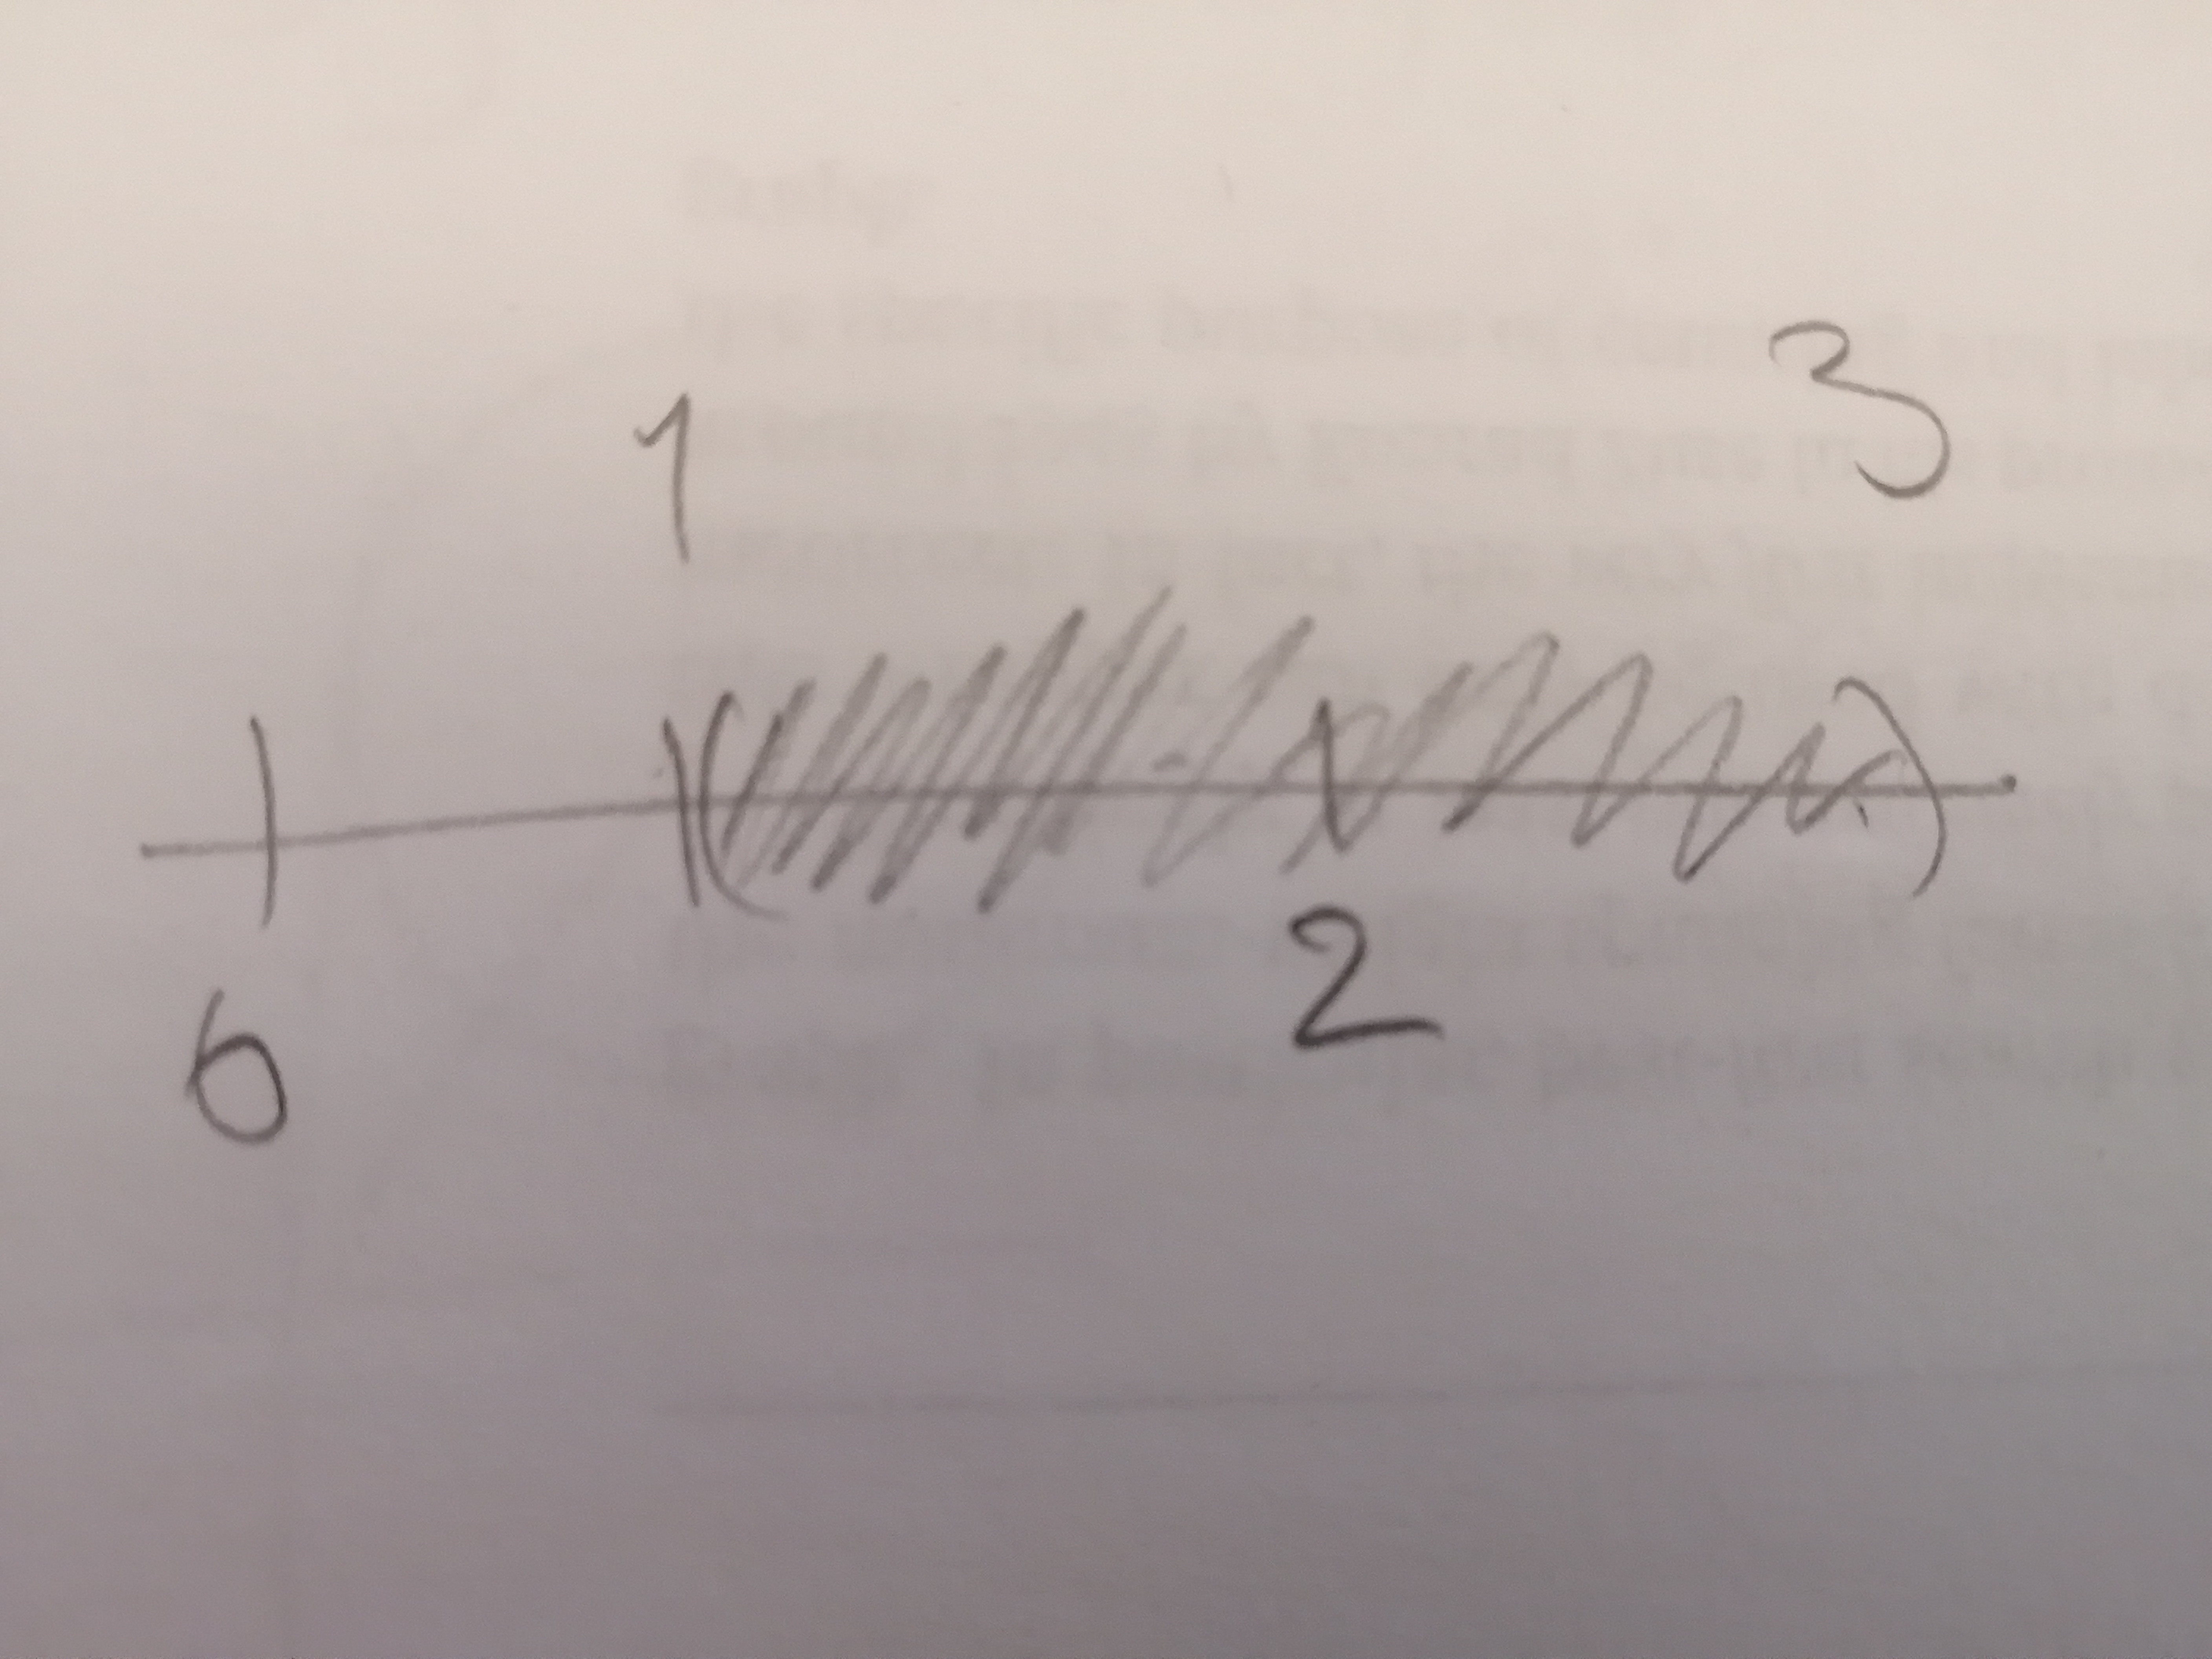
\includegraphics[width=50mm]{assets/lec3_ball-1d.jpg} 
        \end{center}
    \item For these examples notice that there is no outer edge, like an onion with a thin layer peeled off.
\end{itemize}

\newpage

\begin{defn}[Closed Ball]\index{Closed Ball}\label{defn:closed_ball}
    The closed ball centered at $a$,  and radius $r$ is 
    \[
    \bar{B} \left(a, r\right) \coloneqq \left\{ x\in \mathbb{R} ^{n} : \left\Vert a - x \right\Vert \le r \right\} 
    \]
    Notice this differs from the open ball since it contains boundary points.
\end{defn}

\begin{defn}[Sphere]\index{Sphere}\label{defn:sphere}
    The sphere with center $a$ and radius $r$ is 
    \[
    S\left(a, r\right) \coloneqq \left\{ x\in \mathbb{R} ^{n} : \left\Vert x - a \right\Vert = r \right\} 
    \]
    This is only the boundary points now.
\end{defn}

\begin{defn}[Bounded]\index{Bounded}\label{defn:bounded}
    Let $S \subseteq \mathbb{R} ^{n} $, $S$ is bounded if there exists $r > 0$ such that $S  \subseteq B\left(\vec{0} , r\right) $ formally that is 
    \[
    \exists r > 0, \forall x \in S, \left\Vert x \right\Vert \le r
    \]
    It's contained within an open ball.
    \begin{center}
        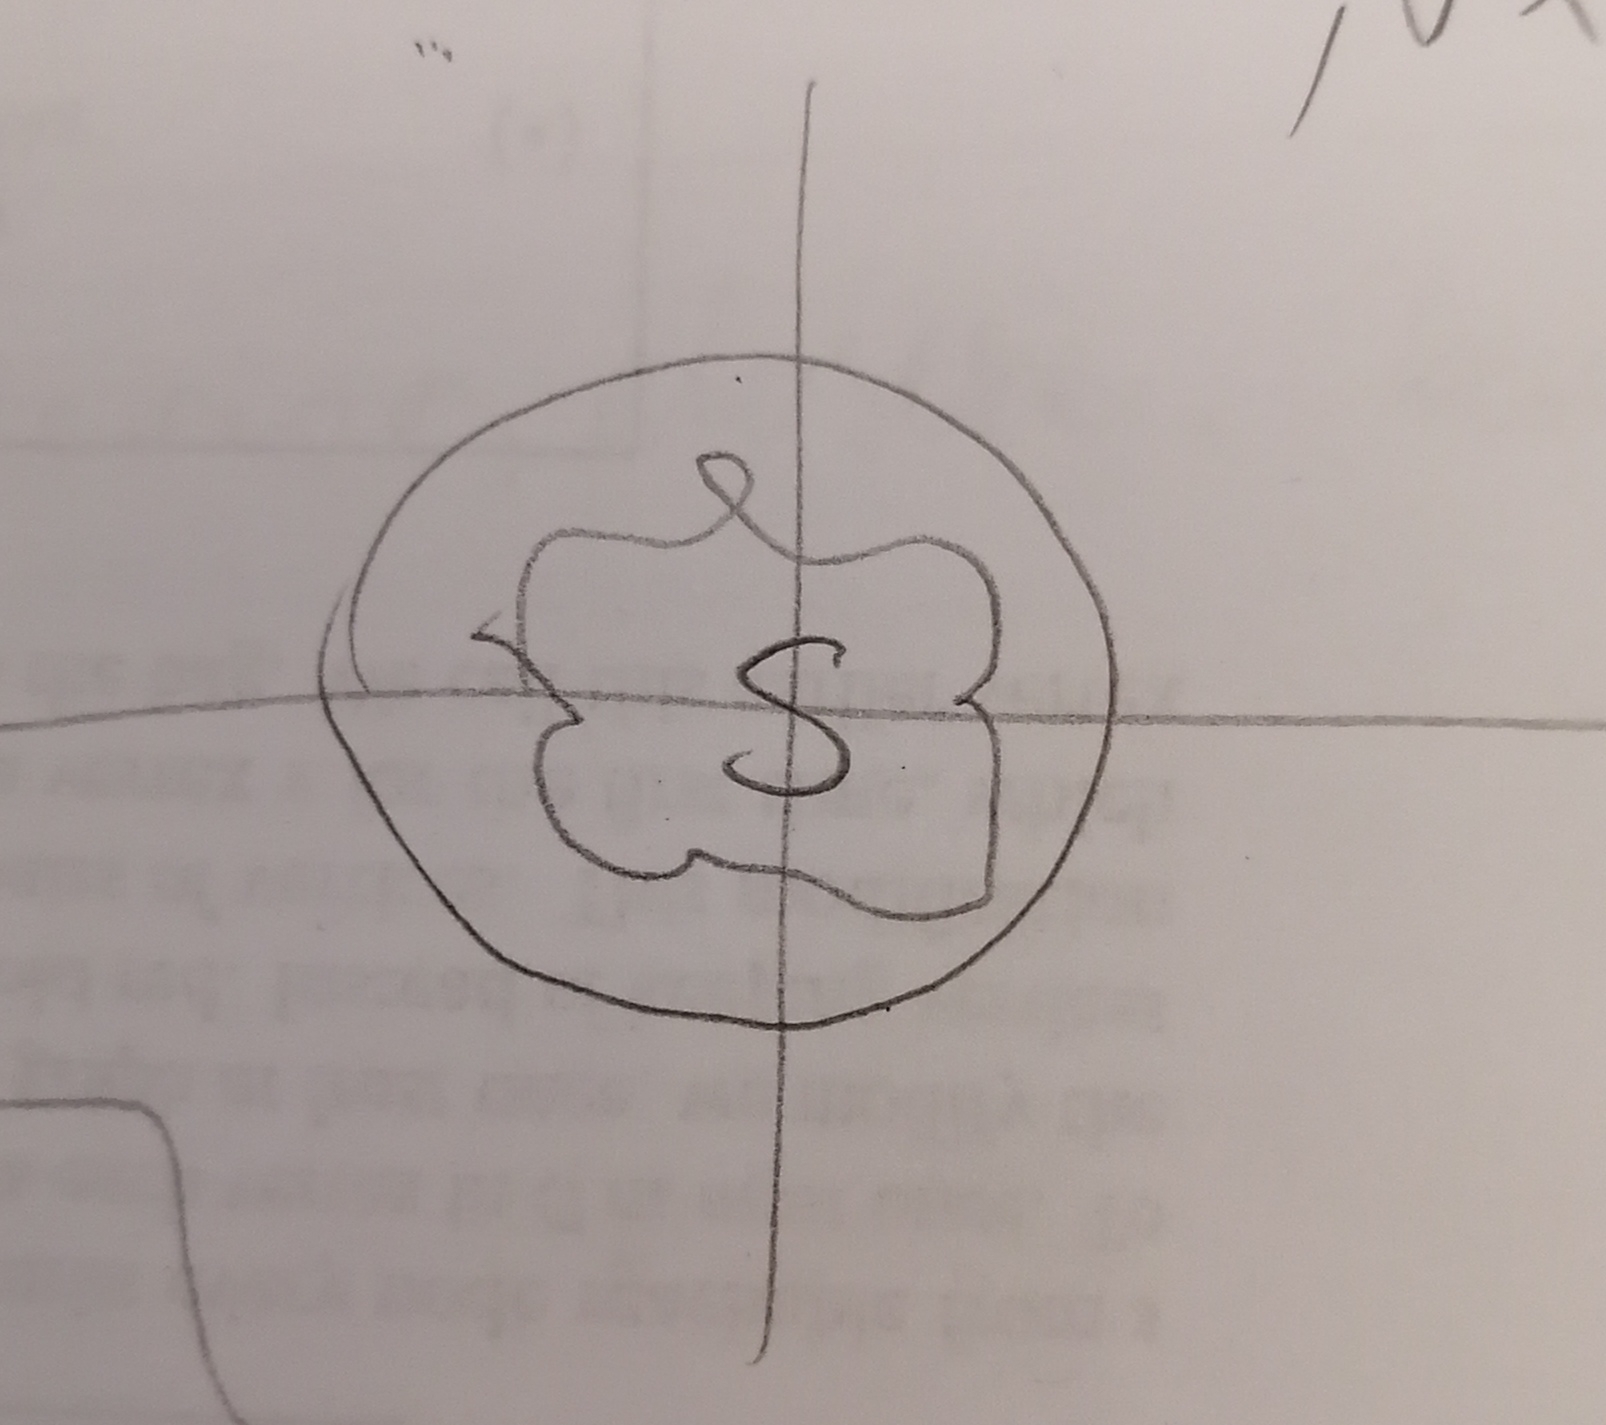
\includegraphics[width=25mm]{assets/lec3-bounded.jpg} 
    \end{center}
\end{defn}

\paragraph{Example} 
We will prove $B\left(a, r\right) \subseteq \mathbb{R} ^{m} $ is bounded.

Intuition, geometrically we have 
\begin{center}
    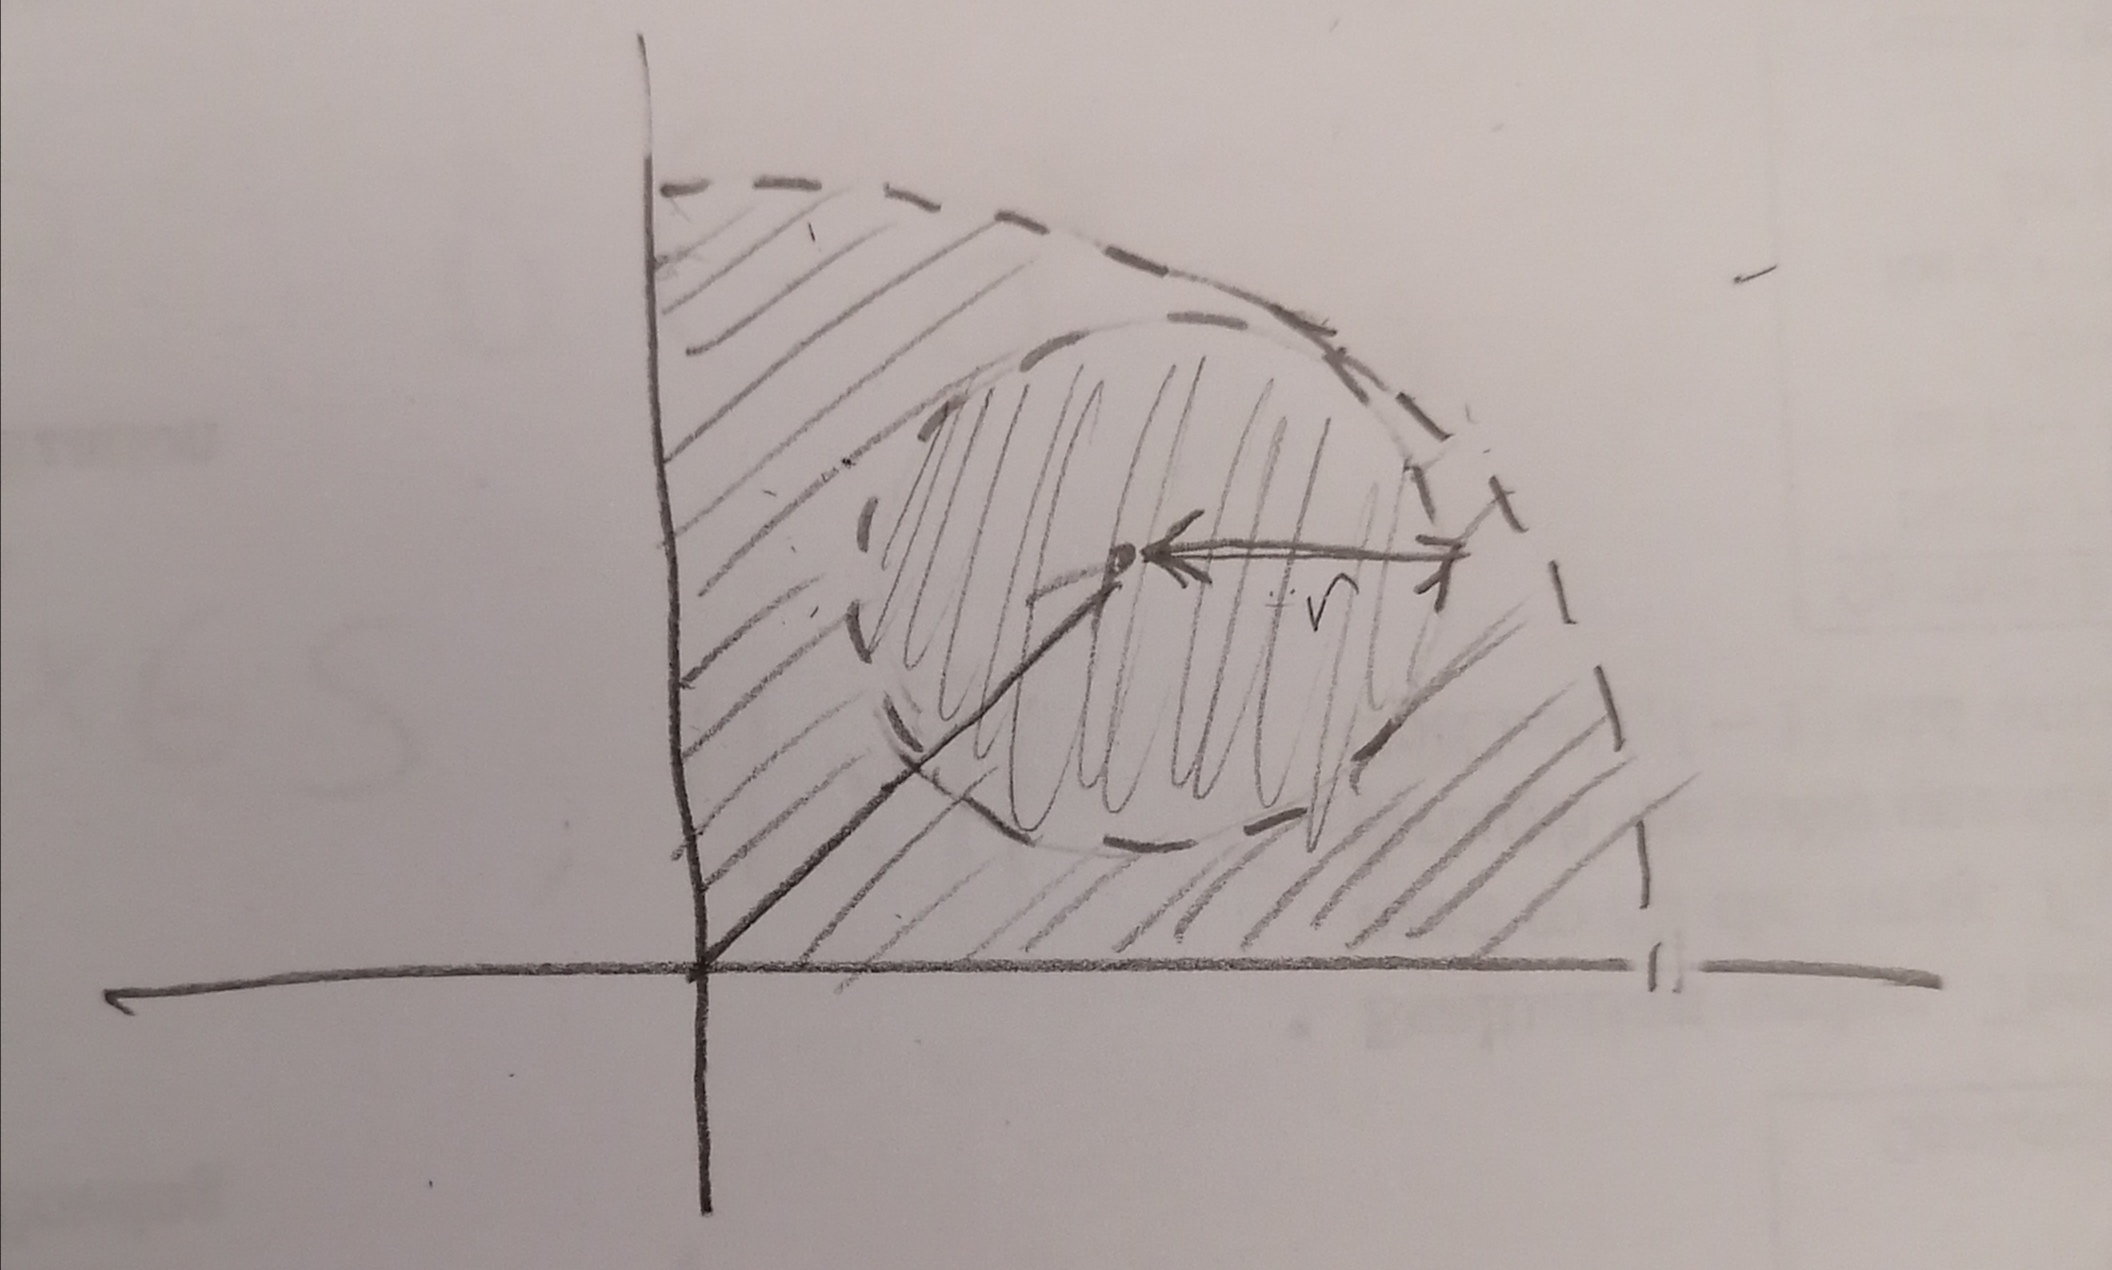
\includegraphics[width=50mm]{assets/lec3-bounded-prf.jpg} 
\end{center}

\paragraph{Rough Work}
\begin{gather}
    \left\Vert a \right\Vert  + r > \left\Vert x - a \right\Vert  + \left\Vert a \right\Vert \\
    \intertext{From the triangle inequality}
    \left\Vert x - a \right\Vert  + \left\Vert a \right\Vert \ge \left\Vert x \right\Vert = \left\Vert x \right\Vert 
\end{gather}

\begin{proof}
$ $\newline
    The set that bounds $B\left(a, r\right) $ is $B\left(a, r  + \left\Vert a \right\Vert \right) $ .Let $x \in B\left(\vec{0} , r\right) $ by definition we need to show that $\left\Vert x \right\Vert \le r + \left\Vert a \right\Vert $ we have 
    \begin{align*}
        \left\Vert x \right\Vert &= \left\Vert x  - a  + a \right\Vert \\
        &\le \left\Vert x - a \right\Vert  + \left\Vert a \right\Vert    \\ 
        &< r  + \left\Vert a \right\Vert    \\ 
    \end{align*}
\end{proof}

\begin{defn}[Interior Point]\index{Interior Point}\label{defn:interior_point}
    We say that $x \in \mathbb{R} ^{m} $ is an interior point of $S$ if 
    \[
    \exists \varepsilon  > 0, B\left(x, \varepsilon \right) \subseteq S
    \]
    This says that if you can have a ball around a point which is completely contained within $S$ then it is on the interior.
\end{defn}

\begin{defn}[Interior]\index{Interior}\label{defn:interior}
    The interior of $S$ is 
    \[
        \mathring{S} \coloneqq \left\{ x\in \mathbb{R} ^{n} : \exists \varepsilon  > 0, B\left(x, \varepsilon \right) \subseteq S \right\} 
    \]
    that is the set of all points that are interior to $S$ 
\end{defn}

\newpage

\begin{defn}[Closure Point]\index{Closure Point}\label{defn:closure_point}
    we say that $x \in R^{n} $ is a closure point of $S$ if
    \[
    \forall \varepsilon  > 0, B\left(x, \varepsilon \right) \cap S \neq \emptyset  
    \]
    So points that lay on the boundary or are inside, must necessarily have this property
\end{defn}

\begin{defn}[Closure]\index{Closure}\label{defn:closure}
    The closure of $S$ is
    \[
        \bar{S} \coloneqq \left\{ x \in \mathbb{R} ^{n} : \forall \varepsilon  > 0, B\left(x, \varepsilon \right) \cap S \neq \emptyset   \right\} 
    \]
    that is, the set of all closure points of $S$ 
\end{defn}

\begin{thm}[Connection between Closure and Interior]\index{Connection between Closure and Interior}\label{thm:connection_between_closure_and_interior}
    For any $S$, we have 
    \[
        \mathring{S} \subseteq S \subseteq \bar{S} 
    \]
\end{thm}

\begin{proof}
$ $\newline
    First we will prove $\mathring{S} \subseteq S$. 
    \begin{itemize}
        \item Let $x \in \mathring{S} $ by definition 
            \[
            \exists \varepsilon _{0}  > 0 \text{ such that } B\left(x, \varepsilon _{0} \right) \subseteq S 
            \]
            But note $x \in B\left(x, \varepsilon _{0} \right) \subseteq S$ therefore $x\in S$
    \end{itemize}
    We will prove $S \subseteq \bar{S} $ 
    \begin{itemize}
        \item let $x \in S$ we know for all $\varepsilon > 0$ that 
            \[
            x\in B\left(x, \varepsilon \right) \cap S
            \]
            so then the intersection of $B\left(x, \varepsilon \right) \cap S \neq 0 $ so $x \in \bar{S} $ 
    \end{itemize}
\end{proof}

\newpage

\begin{defn}[Boundary]\index{Boundary}\label{defn:boundary}
    The boundary of $S$ is 
    \[
    \partial S \coloneqq \bar{S} \setminus \mathring{S} 
    \]
\end{defn}

\subsection{Slide Questions}%
\label{sub:slide_questions}
% subsection slide_questions

\begin{enumerate}
    \item $\mathring{S} = \left( 0,3 \right) , \bar{S} = \left[ 0,3 \right] , \partial S = \left\{ 0,3 \right\} $ 
    \item $\mathring{S} = \left( 0,3 \right) , \bar{S} = \left[ 0,3 \right] , \partial S = \left\{ 0,3 \right\} $ 
    \item $\mathring{S} = \left( 0,3 \right) , \bar{S} = \left[ 0,3 \right] , \partial S = \left\{ 0,3 \right\} $ 
    \item $\mathring{S} = \left( 0,3 \right) , \bar{S} = \left[ 0,3 \right] , \partial S = \left\{ 0,3 \right\} $ 
    \item $\mathring{S} = \emptyset , \bar{S} = \left\{ 0, 3 \right\} , \partial S= \left\{ 0, 3 \right\}  $ 
    \item $\mathring{S} = \mathbb{R} \setminus \left\{ 0 \right\} , \bar{S} = \mathbb{R} = \left\{ 0 \right\} $
    \item $\mathring{S} = \left(  - \infty , 0 \right), \bar{S} = (  - \infty , 0] , \partial S = \left\{ 0 \right\} $ 
    \item $\mathring{S} = \left(  - \infty ,0 \right) \cup \left( 3, \infty  \right), \bar{S} = (n\infty , 0] \cup [3, \infty ) , \partial S = \left\{ 0, 3 \right\} $ 
    \item $\mathring{S} = \left( 0, 3 \right) \times \left\{ 0 \right\}, \bar{S} = \left[ 0, 3 \right] \times \left\{ 0 \right\} , \partial S = \left\{ \left( 0, 0 \right) , \left( 3, 0 \right)  \right\}   $ 
    \item First we go geometric
        \begin{center}
            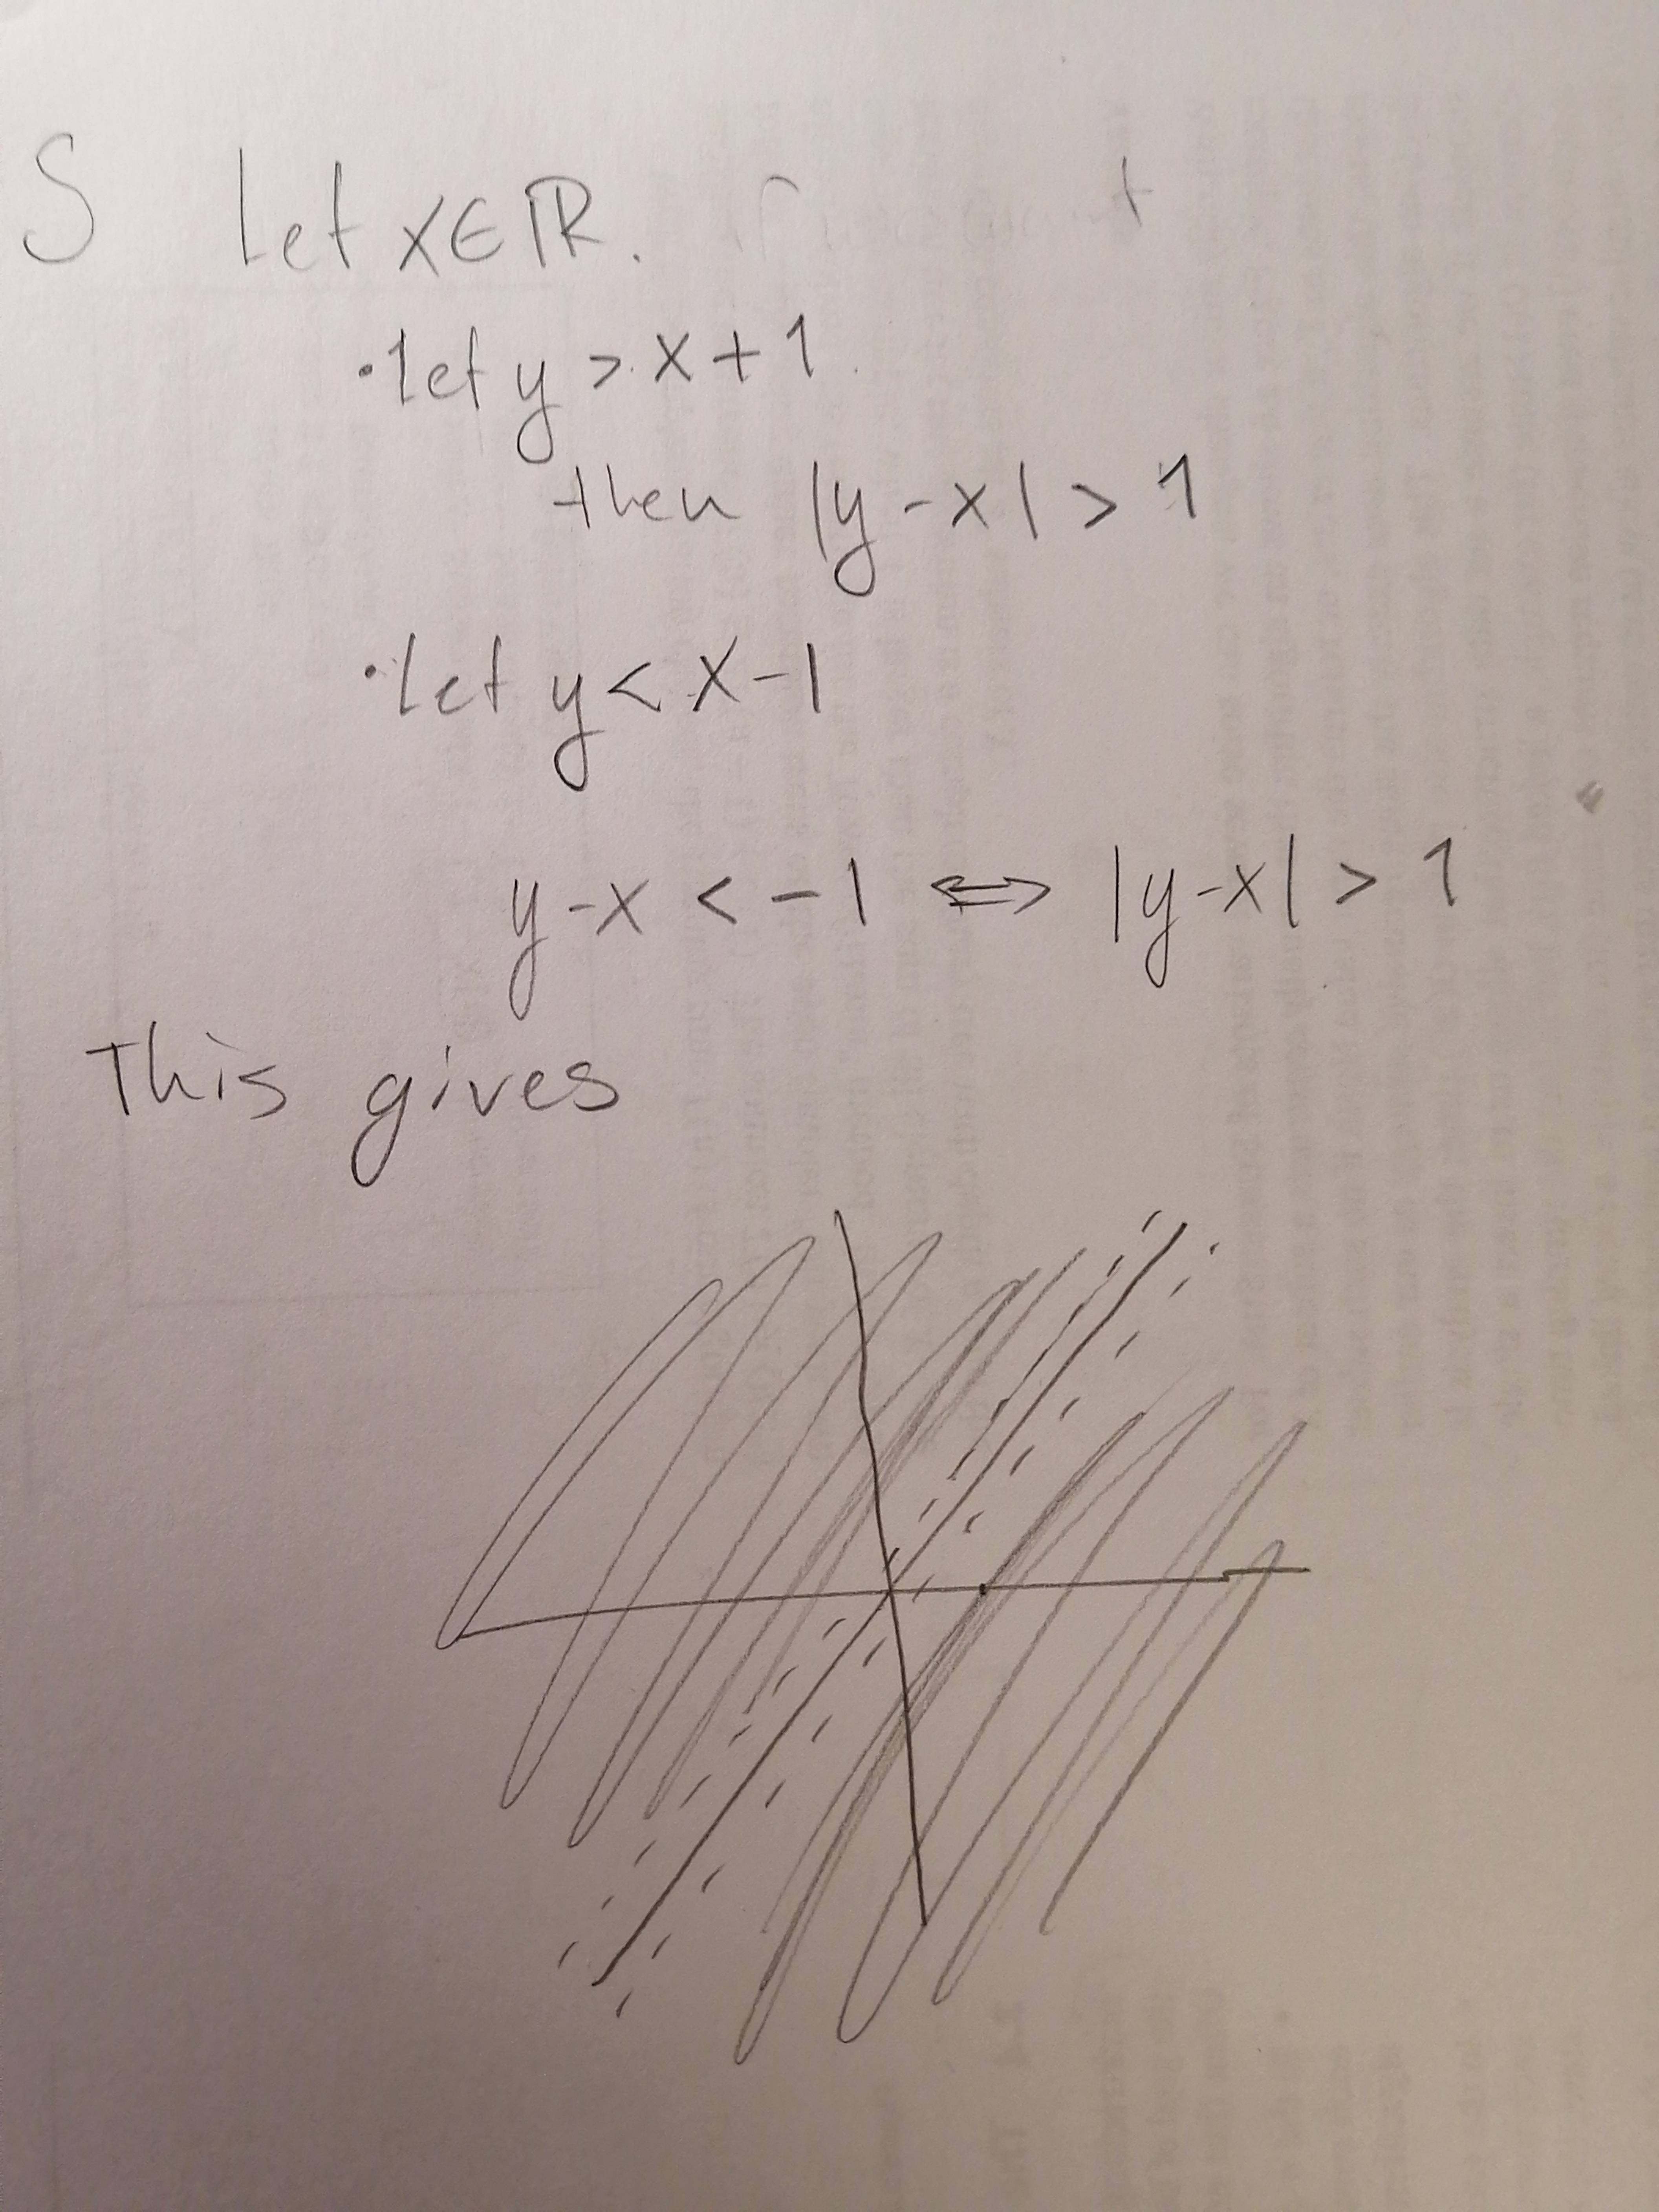
\includegraphics[width=100mm]{assets/lec3-graph.jpg} 
        \end{center}
        So $\mathring{S} = S, ,\bar{S} = \left\{ \left( x,y \right) \in \mathbb{R} ^2 : \left| y - x \right| \ge  1 \right\}, \partial S= \left\{ \left( x,y \right) \in \mathbb{R} ^2 : \left| y - x \right| = 1 \right\} $ 
    \item Note that we can find $x \in \mathbb{Q} $ as small as we want, so then we get gaps as small as we want, so we get $[0, 1)$ with infinitely small holes in it. So $\mathring{S} = \emptyset , \bar{S} = [0, 1), \partial S = [0, 1)$ 
    \item $\mathring{S} = B\left(\vec{0} , 1\right) , \bar{S} = \bar{B} \left(\vec{0}, 1 \right) , \partial S= S\left(\vec{0} , 1\right) $ 
    \item $\mathring{S} = \mathbb{R} ^{n} , \bar{S} = \mathbb{R} ^{n} , \partial S = \emptyset $ 
    \item We know that no element is in $\emptyset $ so clearly no ball contained within $\emptyset $ so $\mathring{S} = \emptyset $,  Also the intersection of anything and $\emptyset $ is also empty so $\bar{S} = \emptyset $,  $\partial S= \emptyset $ 
\end{enumerate}

% subsection slide_questions (end)

% section topology (end)

\chapter{Homework Week 1}%
\label{chp:homework_week_1}
% chapter homework_week_1

\begin{enumerate}
    \item We know that $T_{A}  : R^{7}  \to R^{6}  $ and that $\mathit{null} \left(A\right) $ is the set of elements from $\mathbb{R} ^{7} $ that get mapped to $\vec{0} $
        \begin{enumerate}
            \item So $\mathit{null} \left(A\right) \subseteq \mathbb{R} ^{7} $ 
            \item elements  of the null space are in $\mathbb{R} ^{7} $ no chance to be a sub space in $\mathbb{R} ^{6} $ 
            \item The codomain is what it outputs, we already knwo it is a subset of the domain .
        \item Yes, the null space is a sub space also note that since $A$ represents a linear transformation that $T_{A} \left(0\right) = 0$ and so $A\vec{0} = 0$ and so $\vec{0} \in \mathit{null} \left(A\right) $. 
        \end{enumerate}
    \item If the rank is 4 and the nullspace has dimension 2 by the Rank Nullity Theorem we know there are 6 columns to $A$ the column space is the linear combinations of the columns so if it is a sub space of $\mathbb{R} ^{5} $    that means each column has 5 vertical entries so we can say this matrix is $5 \times 6$ 
    \item Visual Inspection for the rest of the questions
\end{enumerate}

% chapter homework_week_1 (end)

% chapter view (end)

\end{document}
